\documentclass[11pt]{article}
\usepackage[textwidth=18.0cm, textheight=23.0cm, top=2.0cm]{geometry}
\usepackage{pst-all}
\usepackage{amssymb}
\usepackage{tikz}
\usepackage{underscore}\begin{document}
\pagestyle{empty}


ClassName: \underline{\textbf{Class_03.2bp-36}}
\par
BinSize: \underline{\textbf{40 × 40}}
\par
ReduceSize: \underline{\textbf{40 × 40}}
\par
TypeNum: \underline{\textbf{79}}
\par
Num: \underline{\textbf{80}}
\par
OutS: \underline{\textbf{32000}}
\par
InS: \underline{\textbf{29037}}
\par
Rate: \underline{\textbf{0.907}}
\par
UB: \underline{\textbf{20}}
\par
LB0: \underline{\textbf{20}}
\par
LB: \underline{\textbf{20}}
\par
LBWithCut: \underline{\textbf{20}}
\par
NodeCut: \underline{\textbf{0}}
\par
ExtendedNodeCnt: \underline{\textbf{1}}
\par
GenNodeCnt: \underline{\textbf{1}}
\par
PrimalNode: \underline{\textbf{0}}
\par
ColumnCount: \underline{\textbf{20}}
\par
TotalCutCount: \underline{\textbf{0}}
\par
RootCutCount: \underline{\textbf{0}}
\par
LPSolverCnt: \underline{\textbf{1}}
\par
PricingSolverCnt: \underline{\textbf{0}}
\par
BranchAndBoundNum: \underline{\textbf{1}}
\par
isOpt: \underline{\textbf{true}}
\par
TimeOnInitSolution: \underline{\textbf{17.830 s}}
\par
TimeOnPrimal: \underline{\textbf{0.000 s}}
\par
TimeOnPricing: \underline{\textbf{0.000 s}}
\par
TimeOnRmp: \underline{\textbf{0.078 s}}
\par
TotalTime: \underline{\textbf{17.971 s}}
\par
\newpage


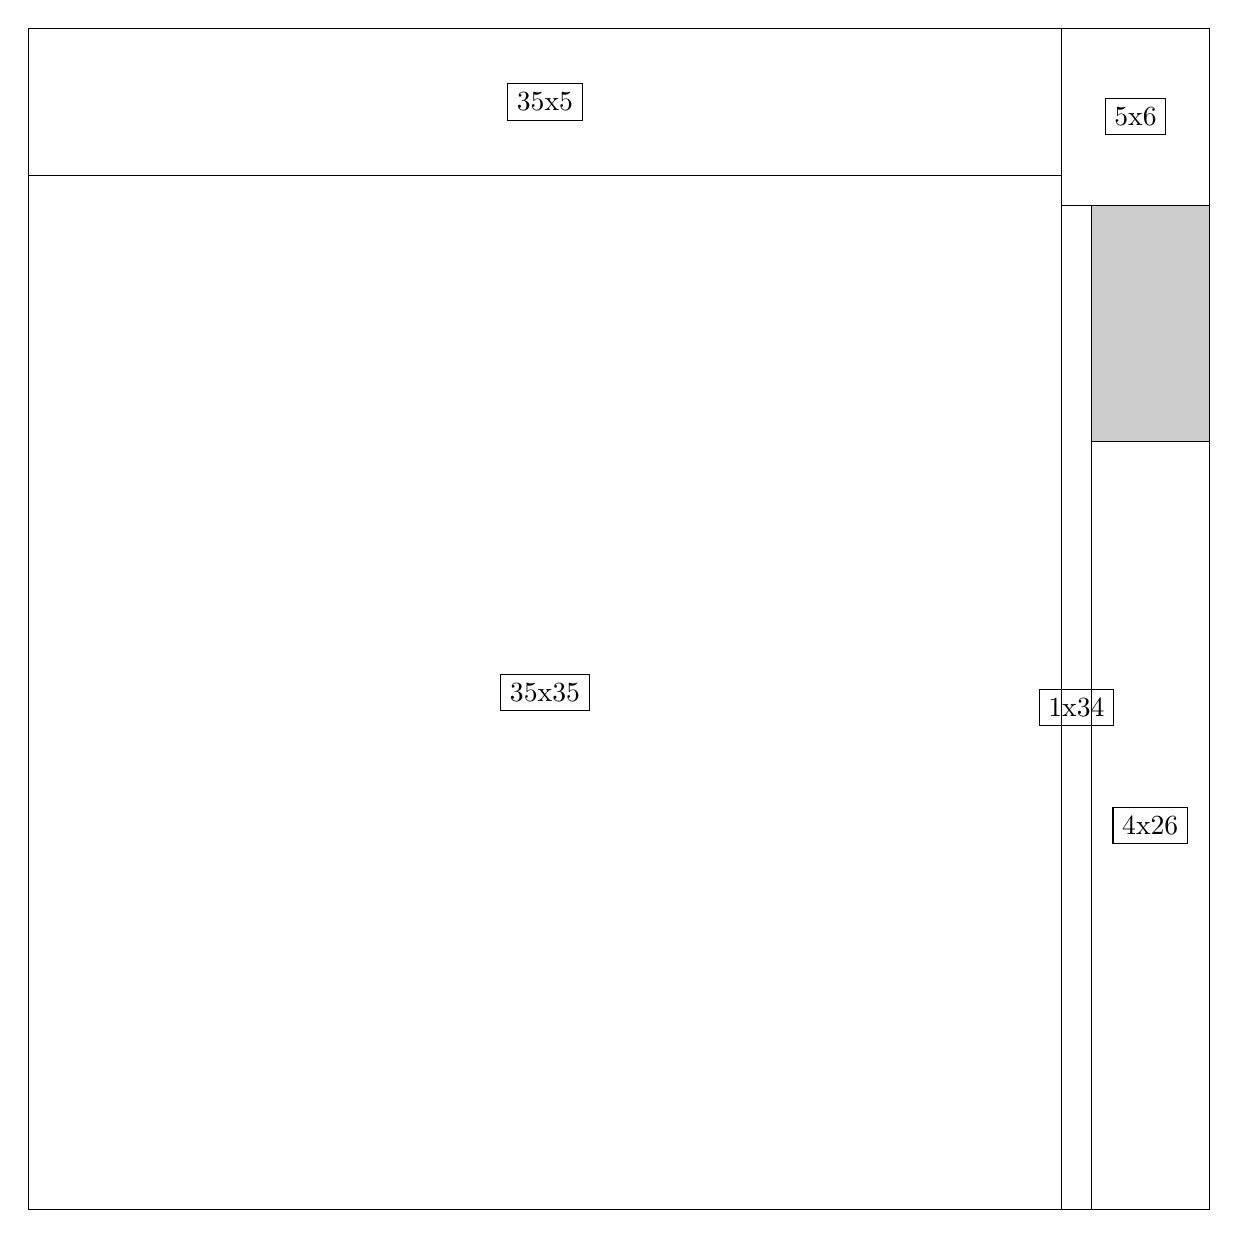
\begin{tikzpicture}[shorten >=1pt,scale=1.0,every node/.style={scale=1.0},->]
\tikzstyle{vertex}=[circle,fill=black!25,minimum size=14pt,inner sep=0pt]
\filldraw[fill=gray!40!white, draw=black] (0,0) rectangle (15.0,15.0);
\foreach \name/\x/\y/\w/\h in {35x35/0.0/0.0/13.125/13.125,35x5/0.0/13.125/13.125/1.875,4x26/13.5/0.0/1.5/9.75,1x34/13.125/0.0/0.375/12.75,5x6/13.125/12.75/1.875/2.25}
\filldraw[fill=white!40!white, draw=black] (\x,\y) rectangle node[draw] (\name) {\name} ++(\w,\h);
\end{tikzpicture}


w =35 , h =35 , x =0 , y =0 , v =1225
\par
w =35 , h =5 , x =0 , y =35 , v =175
\par
w =4 , h =26 , x =36 , y =0 , v =104
\par
w =1 , h =34 , x =35 , y =0 , v =34
\par
w =5 , h =6 , x =35 , y =34 , v =30
\par
\newpage


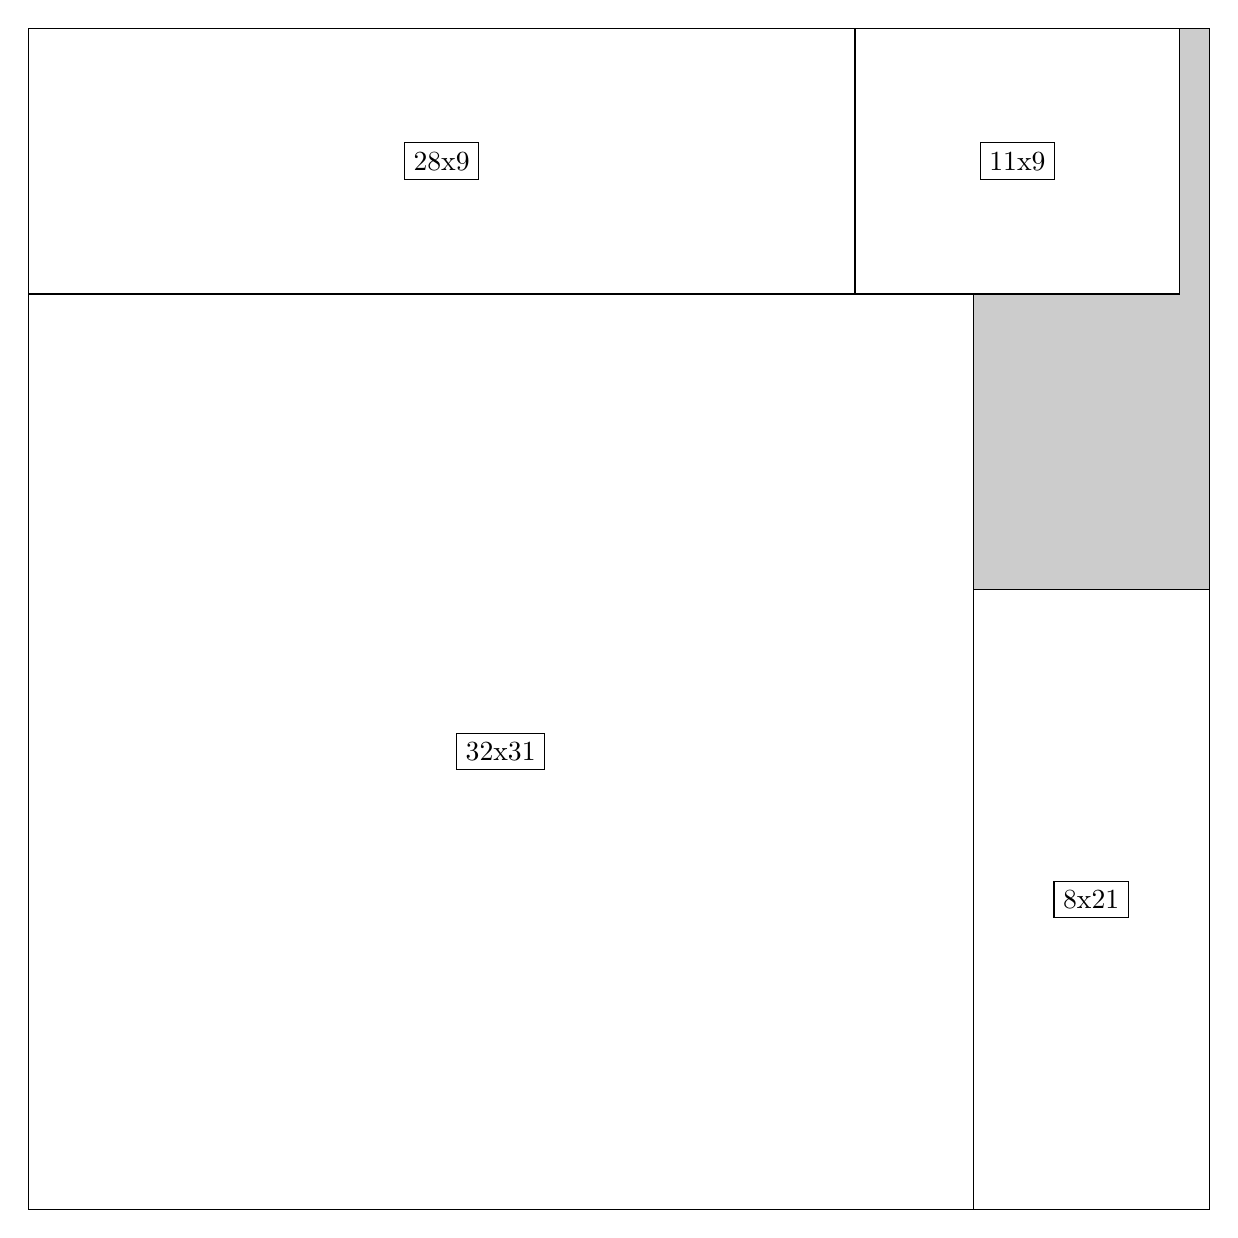
\begin{tikzpicture}[shorten >=1pt,scale=1.0,every node/.style={scale=1.0},->]
\tikzstyle{vertex}=[circle,fill=black!25,minimum size=14pt,inner sep=0pt]
\filldraw[fill=gray!40!white, draw=black] (0,0) rectangle (15.0,15.0);
\foreach \name/\x/\y/\w/\h in {32x31/0.0/0.0/12.0/11.625,28x9/0.0/11.625/10.5/3.375,8x21/12.0/0.0/3.0/7.875,11x9/10.5/11.625/4.125/3.375}
\filldraw[fill=white!40!white, draw=black] (\x,\y) rectangle node[draw] (\name) {\name} ++(\w,\h);
\end{tikzpicture}


w =32 , h =31 , x =0 , y =0 , v =992
\par
w =28 , h =9 , x =0 , y =31 , v =252
\par
w =8 , h =21 , x =32 , y =0 , v =168
\par
w =11 , h =9 , x =28 , y =31 , v =99
\par
\newpage


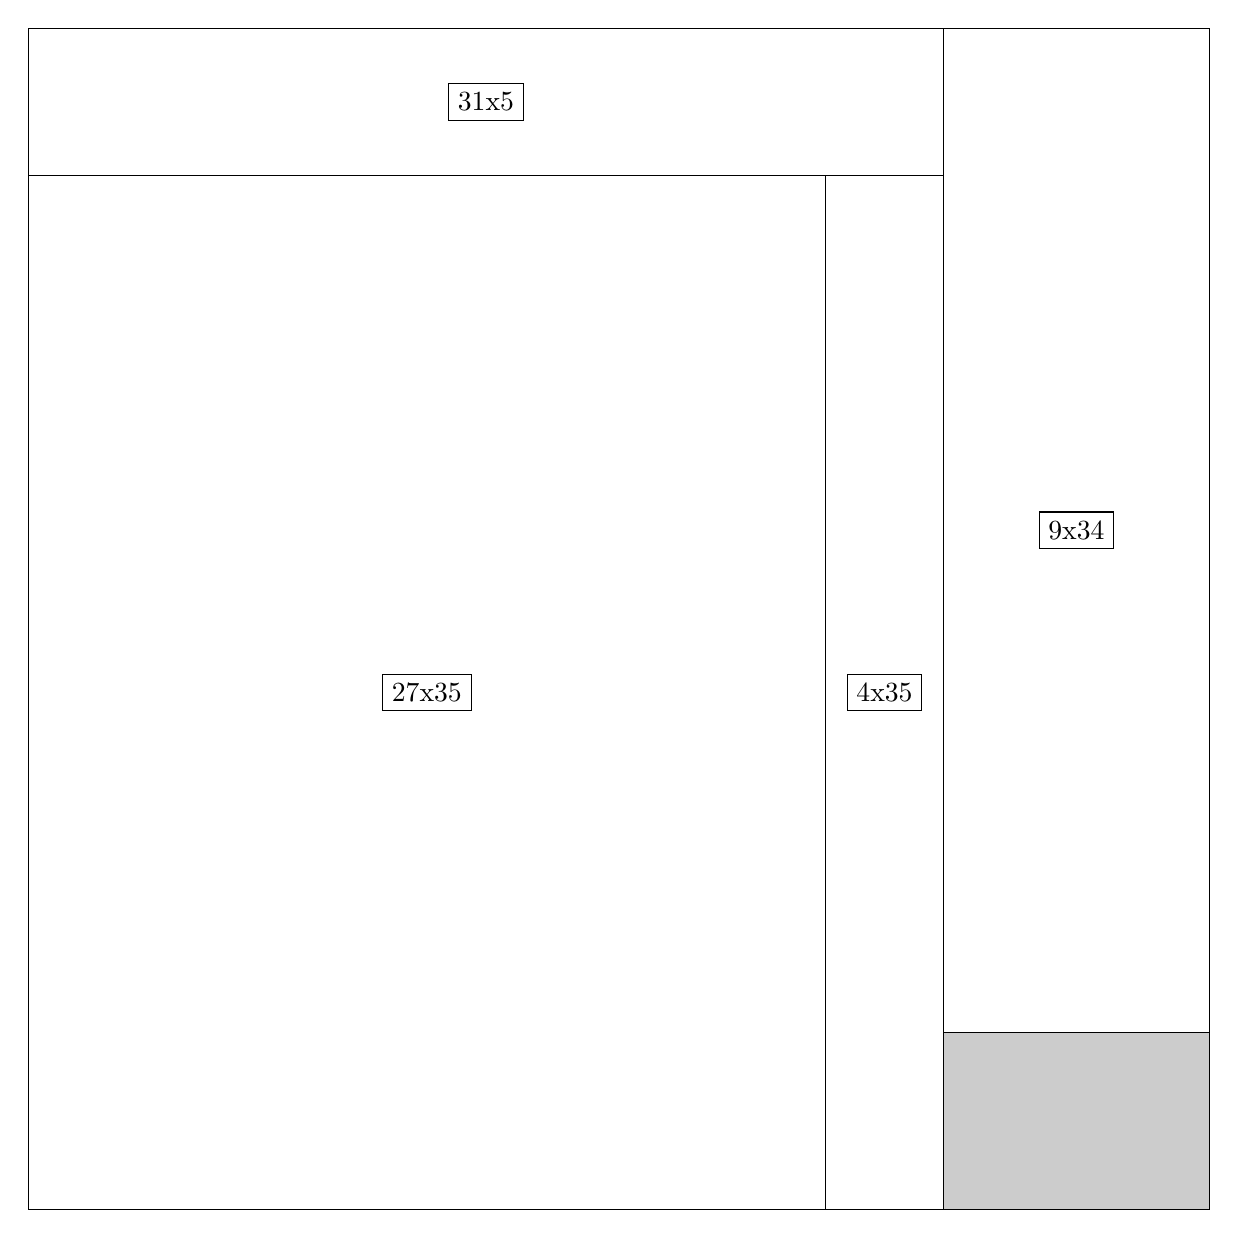
\begin{tikzpicture}[shorten >=1pt,scale=1.0,every node/.style={scale=1.0},->]
\tikzstyle{vertex}=[circle,fill=black!25,minimum size=14pt,inner sep=0pt]
\filldraw[fill=gray!40!white, draw=black] (0,0) rectangle (15.0,15.0);
\foreach \name/\x/\y/\w/\h in {27x35/0.0/0.0/10.125/13.125,31x5/0.0/13.125/11.625/1.875,9x34/11.625/2.25/3.375/12.75,4x35/10.125/0.0/1.5/13.125}
\filldraw[fill=white!40!white, draw=black] (\x,\y) rectangle node[draw] (\name) {\name} ++(\w,\h);
\end{tikzpicture}


w =27 , h =35 , x =0 , y =0 , v =945
\par
w =31 , h =5 , x =0 , y =35 , v =155
\par
w =9 , h =34 , x =31 , y =6 , v =306
\par
w =4 , h =35 , x =27 , y =0 , v =140
\par
\newpage


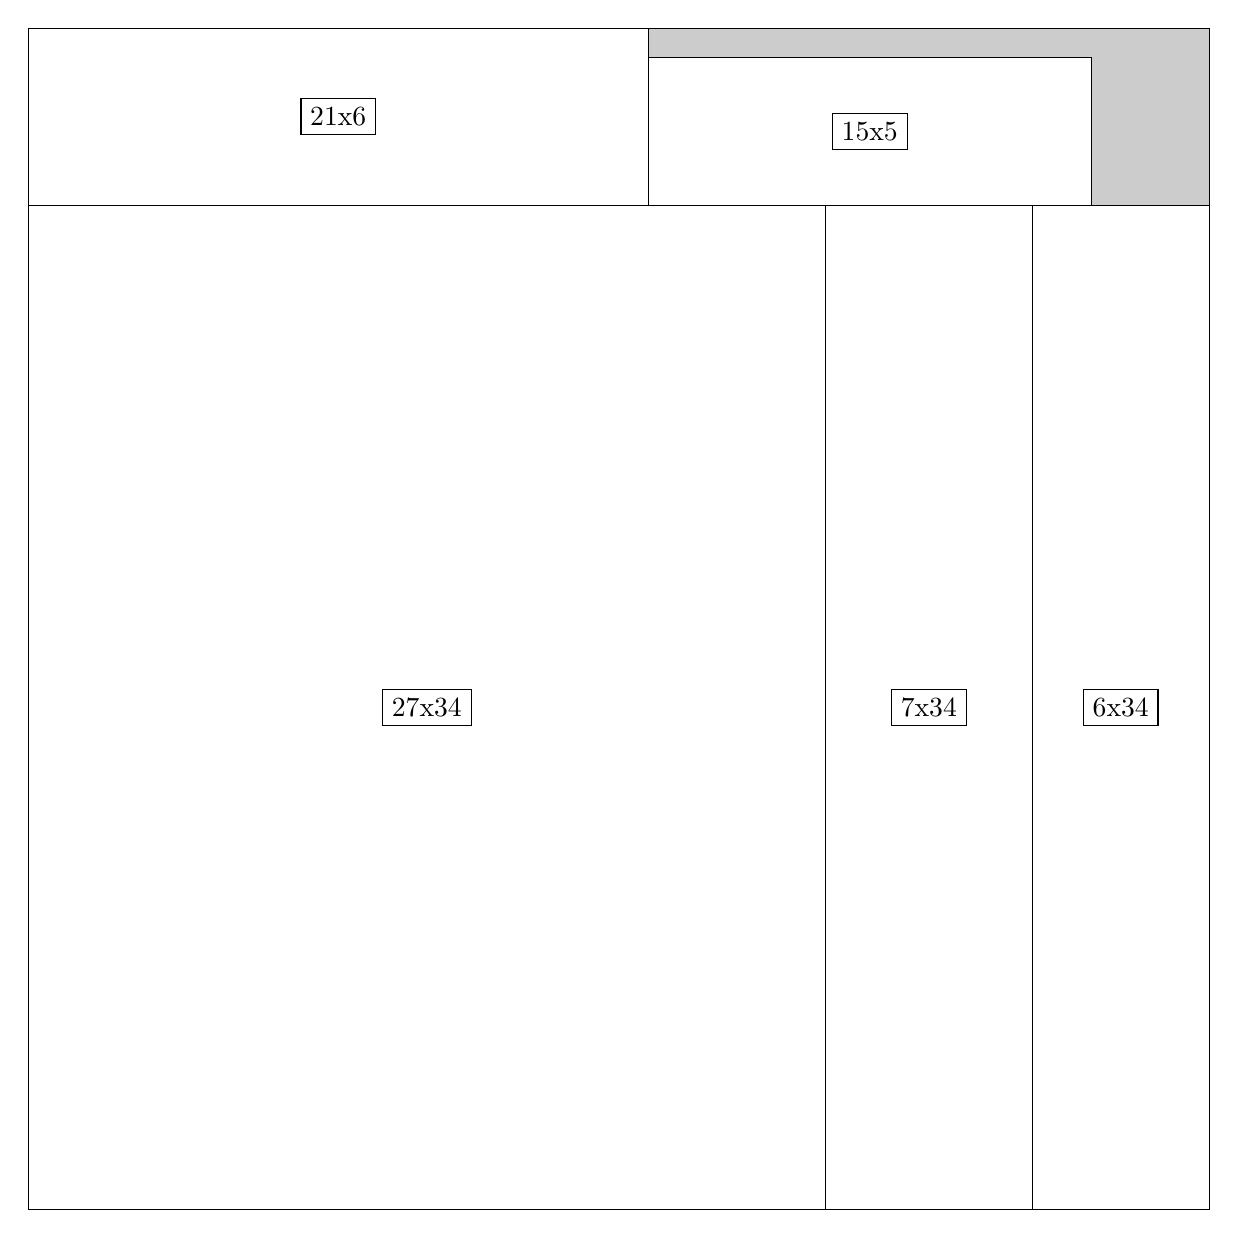
\begin{tikzpicture}[shorten >=1pt,scale=1.0,every node/.style={scale=1.0},->]
\tikzstyle{vertex}=[circle,fill=black!25,minimum size=14pt,inner sep=0pt]
\filldraw[fill=gray!40!white, draw=black] (0,0) rectangle (15.0,15.0);
\foreach \name/\x/\y/\w/\h in {27x34/0.0/0.0/10.125/12.75,7x34/10.125/0.0/2.625/12.75,6x34/12.75/0.0/2.25/12.75,21x6/0.0/12.75/7.875/2.25,15x5/7.875/12.75/5.625/1.875}
\filldraw[fill=white!40!white, draw=black] (\x,\y) rectangle node[draw] (\name) {\name} ++(\w,\h);
\end{tikzpicture}


w =27 , h =34 , x =0 , y =0 , v =918
\par
w =7 , h =34 , x =27 , y =0 , v =238
\par
w =6 , h =34 , x =34 , y =0 , v =204
\par
w =21 , h =6 , x =0 , y =34 , v =126
\par
w =15 , h =5 , x =21 , y =34 , v =75
\par
\newpage


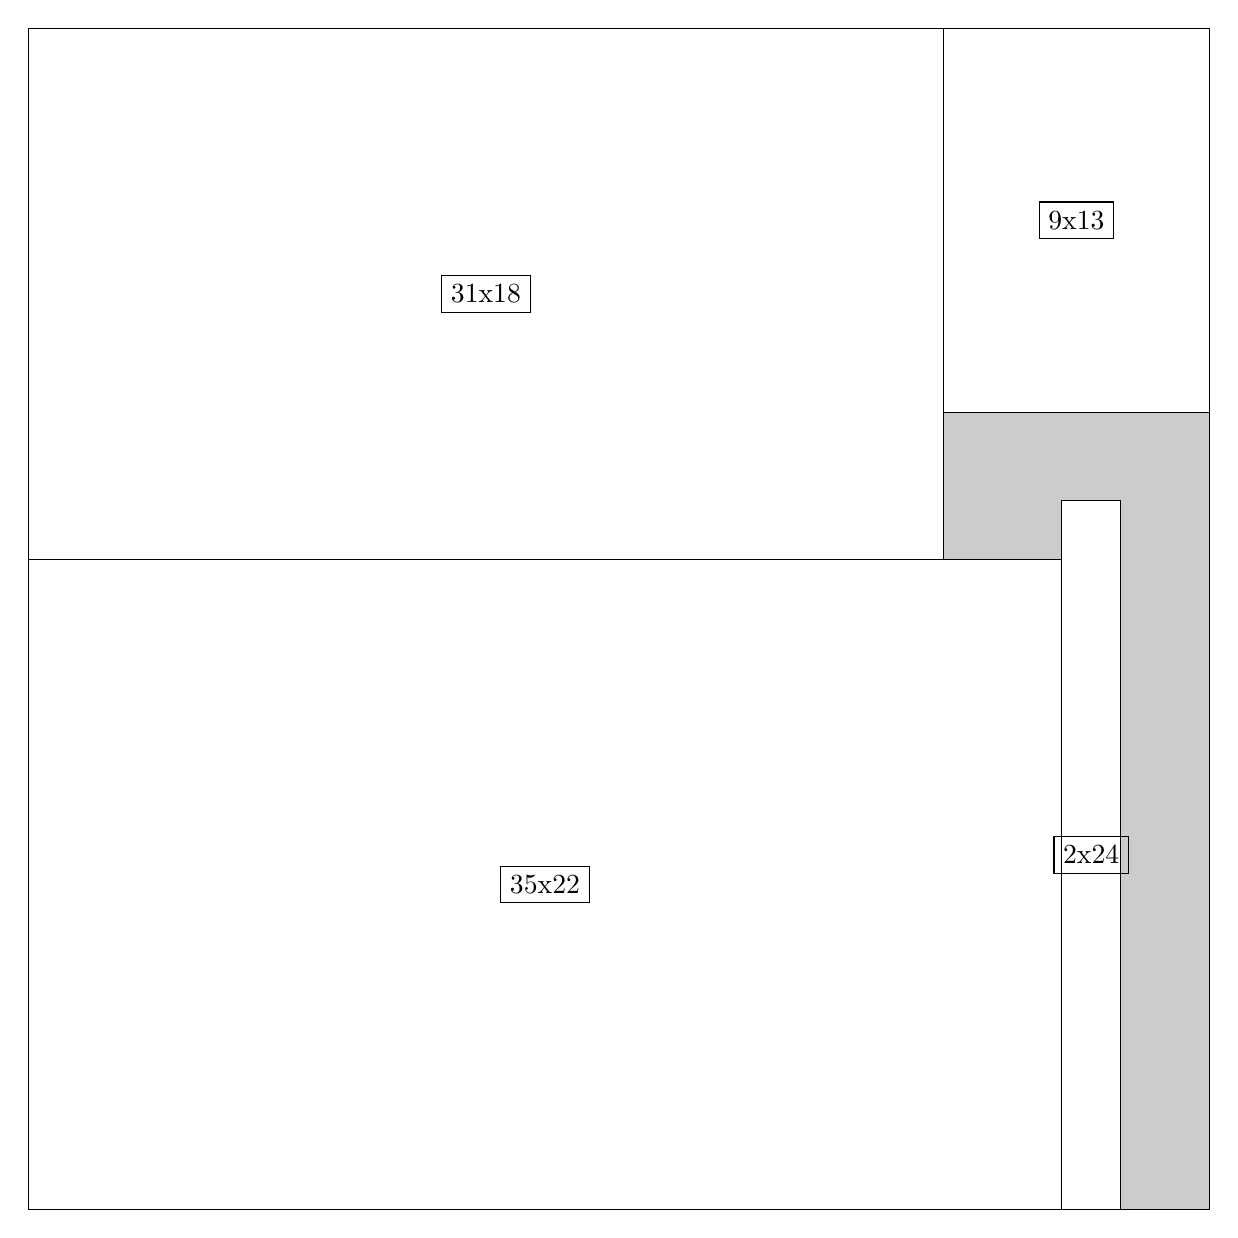
\begin{tikzpicture}[shorten >=1pt,scale=1.0,every node/.style={scale=1.0},->]
\tikzstyle{vertex}=[circle,fill=black!25,minimum size=14pt,inner sep=0pt]
\filldraw[fill=gray!40!white, draw=black] (0,0) rectangle (15.0,15.0);
\foreach \name/\x/\y/\w/\h in {35x22/0.0/0.0/13.125/8.25,31x18/0.0/8.25/11.625/6.75,9x13/11.625/10.125/3.375/4.875,2x24/13.125/0.0/0.75/9.0}
\filldraw[fill=white!40!white, draw=black] (\x,\y) rectangle node[draw] (\name) {\name} ++(\w,\h);
\end{tikzpicture}


w =35 , h =22 , x =0 , y =0 , v =770
\par
w =31 , h =18 , x =0 , y =22 , v =558
\par
w =9 , h =13 , x =31 , y =27 , v =117
\par
w =2 , h =24 , x =35 , y =0 , v =48
\par
\newpage


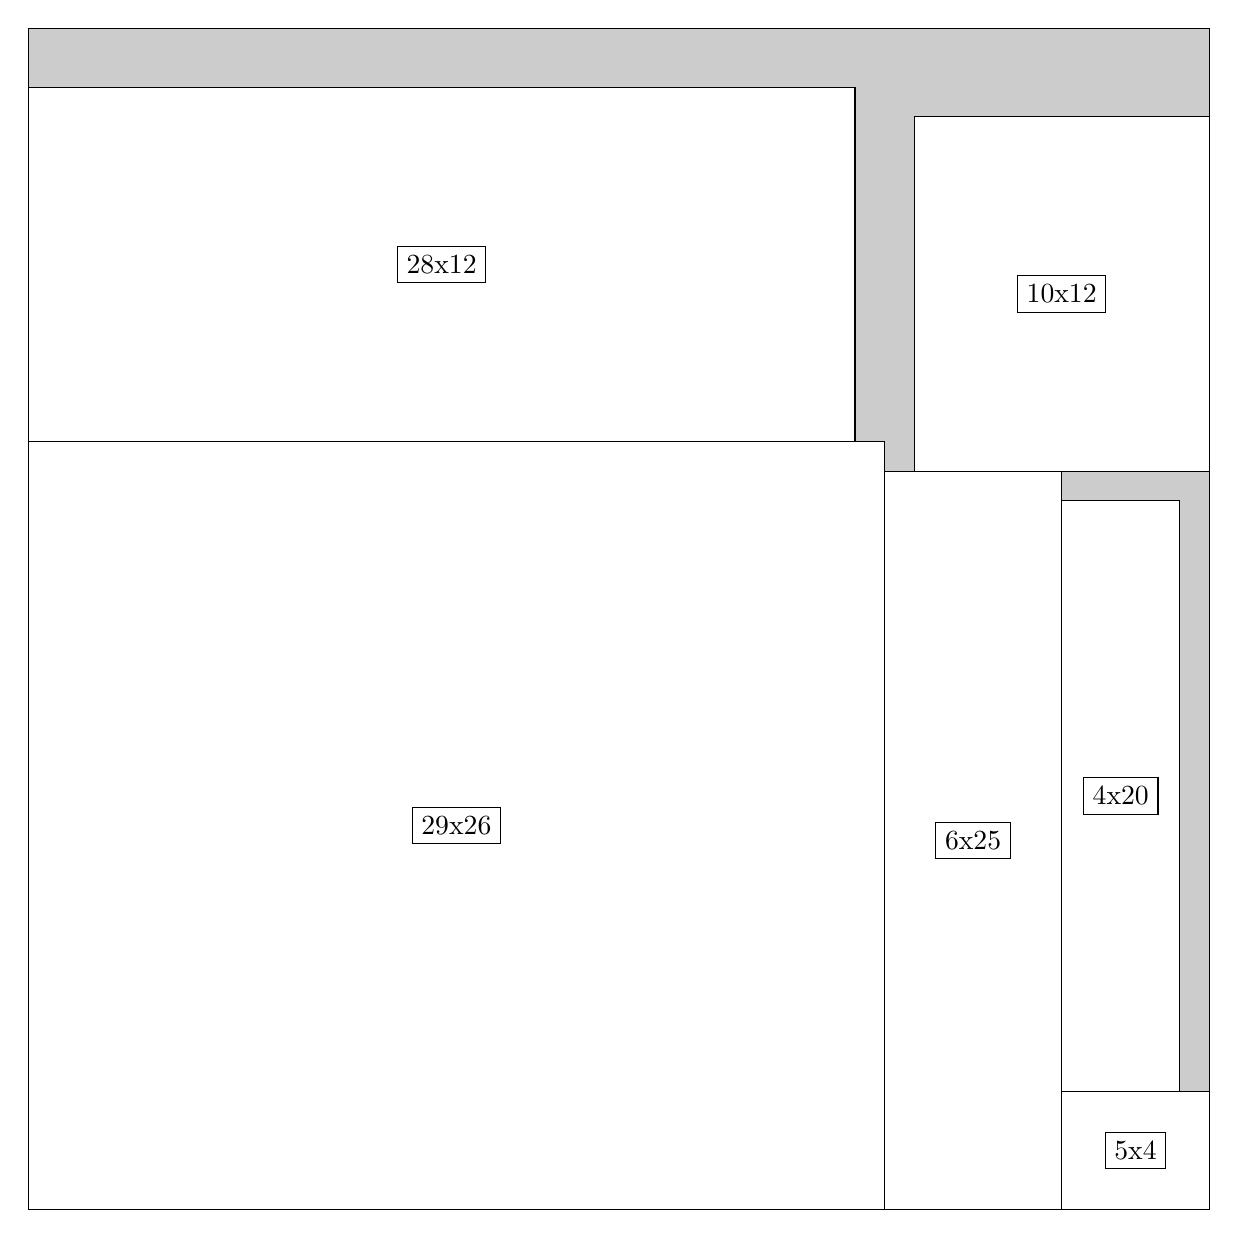
\begin{tikzpicture}[shorten >=1pt,scale=1.0,every node/.style={scale=1.0},->]
\tikzstyle{vertex}=[circle,fill=black!25,minimum size=14pt,inner sep=0pt]
\filldraw[fill=gray!40!white, draw=black] (0,0) rectangle (15.0,15.0);
\foreach \name/\x/\y/\w/\h in {29x26/0.0/0.0/10.875/9.75,6x25/10.875/0.0/2.25/9.375,28x12/0.0/9.75/10.5/4.5,10x12/11.25/9.375/3.75/4.5,4x20/13.125/1.5/1.5/7.5,5x4/13.125/0.0/1.875/1.5}
\filldraw[fill=white!40!white, draw=black] (\x,\y) rectangle node[draw] (\name) {\name} ++(\w,\h);
\end{tikzpicture}


w =29 , h =26 , x =0 , y =0 , v =754
\par
w =6 , h =25 , x =29 , y =0 , v =150
\par
w =28 , h =12 , x =0 , y =26 , v =336
\par
w =10 , h =12 , x =30 , y =25 , v =120
\par
w =4 , h =20 , x =35 , y =4 , v =80
\par
w =5 , h =4 , x =35 , y =0 , v =20
\par
\newpage


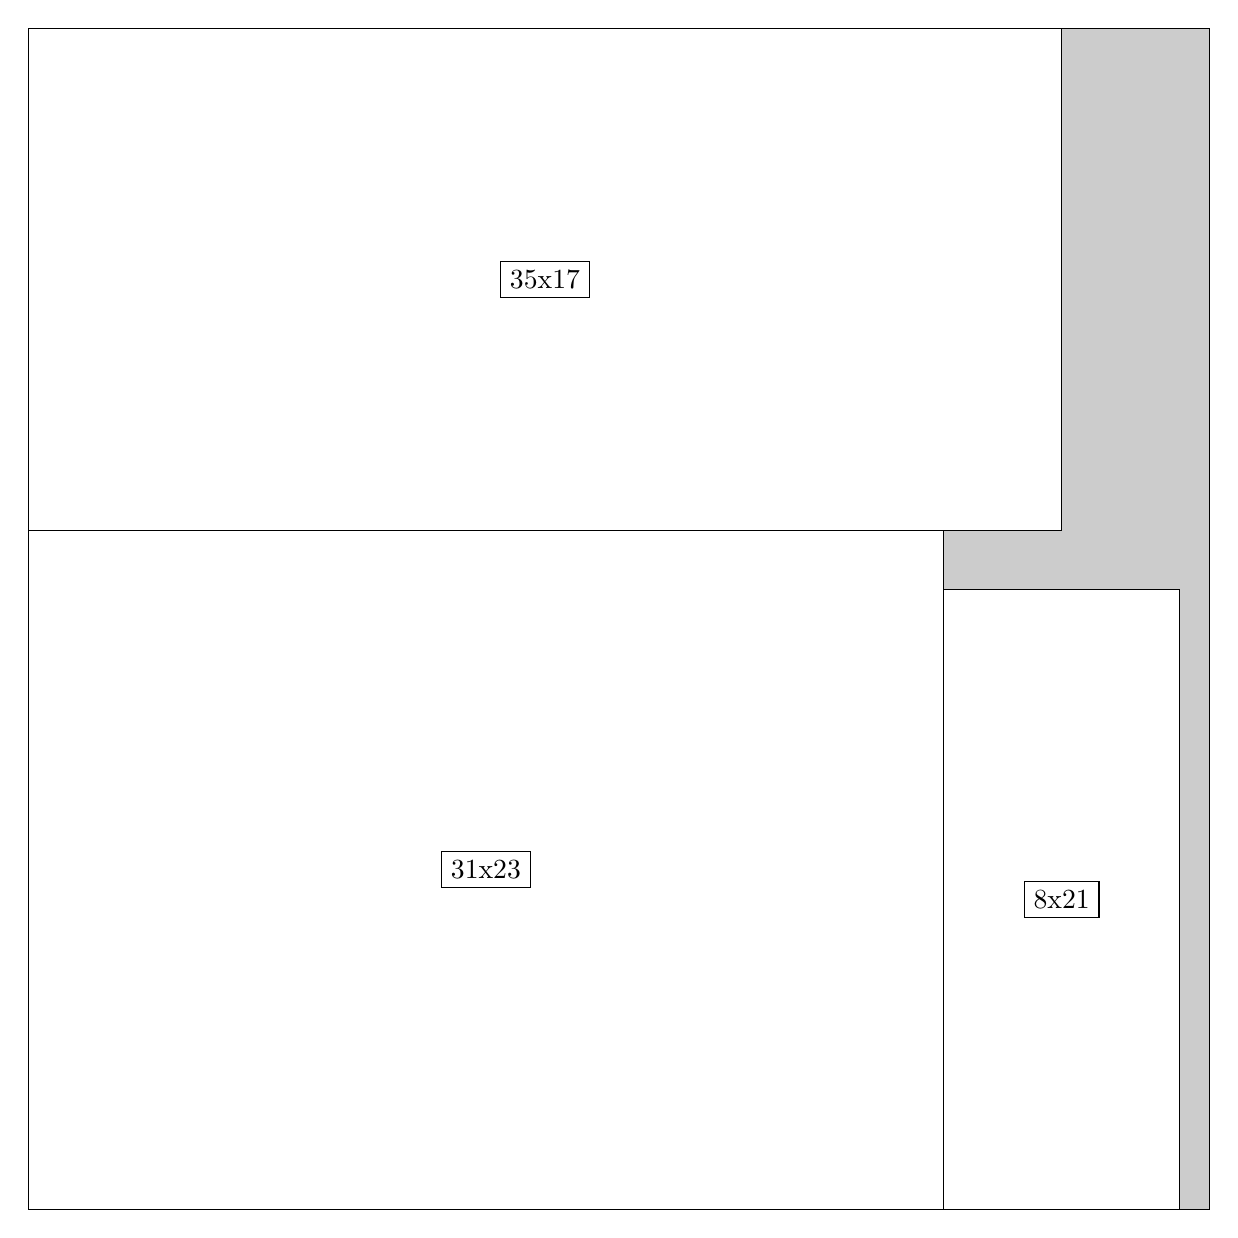
\begin{tikzpicture}[shorten >=1pt,scale=1.0,every node/.style={scale=1.0},->]
\tikzstyle{vertex}=[circle,fill=black!25,minimum size=14pt,inner sep=0pt]
\filldraw[fill=gray!40!white, draw=black] (0,0) rectangle (15.0,15.0);
\foreach \name/\x/\y/\w/\h in {35x17/0.0/8.625/13.125/6.375,8x21/11.625/0.0/3.0/7.875,31x23/0.0/0.0/11.625/8.625}
\filldraw[fill=white!40!white, draw=black] (\x,\y) rectangle node[draw] (\name) {\name} ++(\w,\h);
\end{tikzpicture}


w =35 , h =17 , x =0 , y =23 , v =595
\par
w =8 , h =21 , x =31 , y =0 , v =168
\par
w =31 , h =23 , x =0 , y =0 , v =713
\par
\newpage


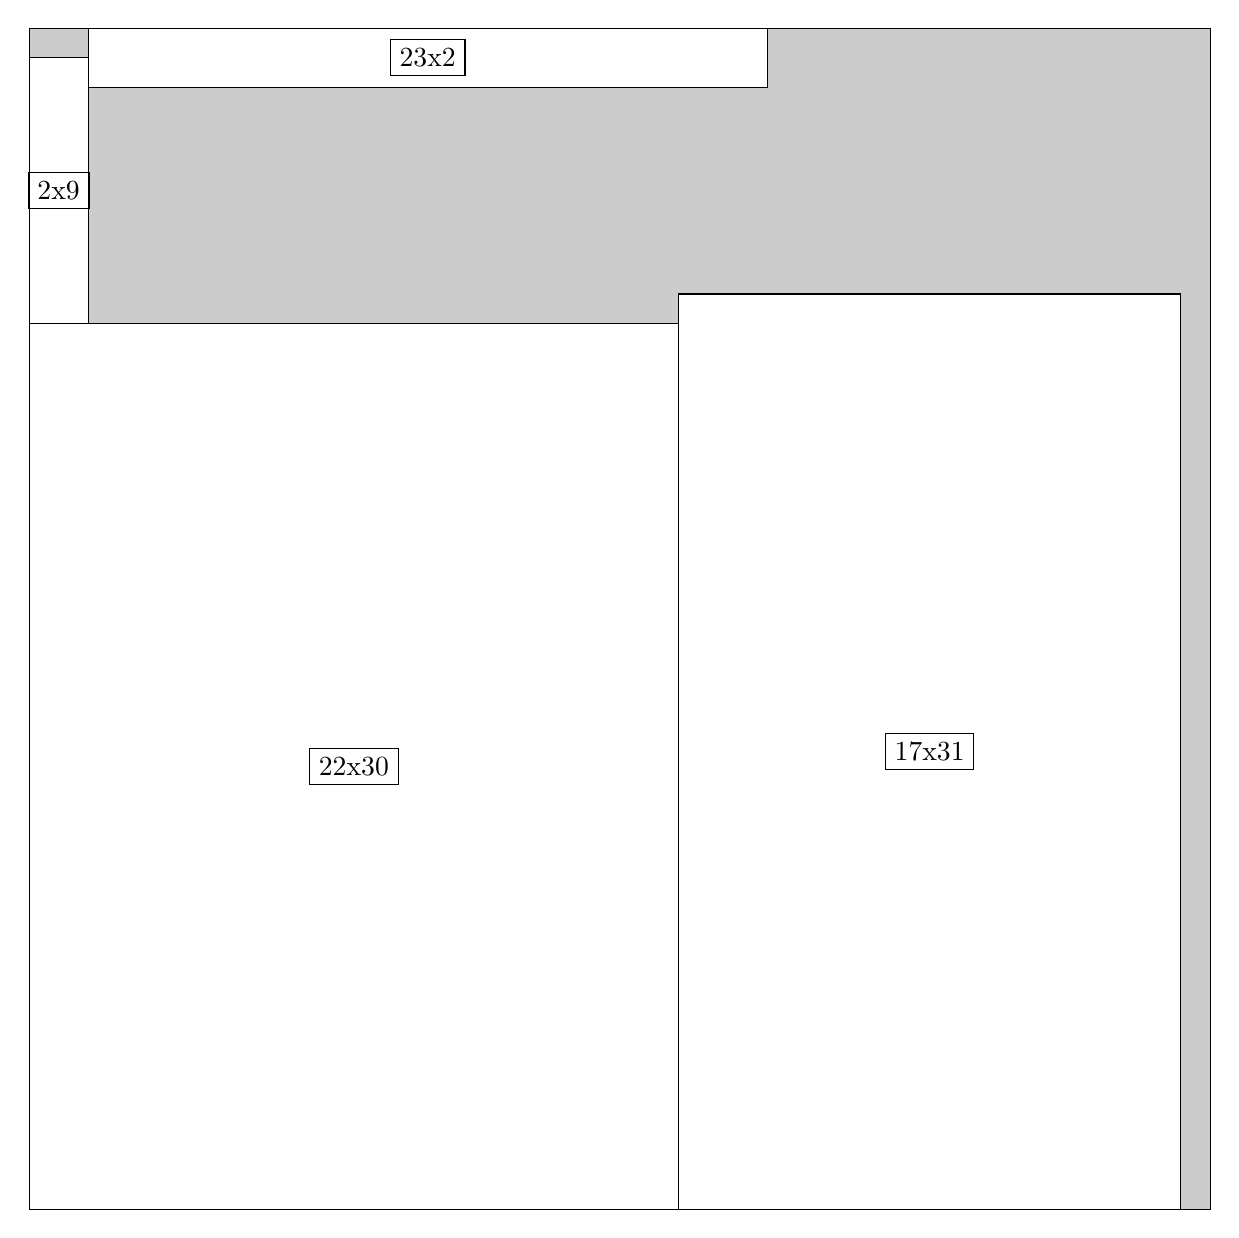
\begin{tikzpicture}[shorten >=1pt,scale=1.0,every node/.style={scale=1.0},->]
\tikzstyle{vertex}=[circle,fill=black!25,minimum size=14pt,inner sep=0pt]
\filldraw[fill=gray!40!white, draw=black] (0,0) rectangle (15.0,15.0);
\foreach \name/\x/\y/\w/\h in {22x30/0.0/0.0/8.25/11.25,17x31/8.25/0.0/6.375/11.625,23x2/0.75/14.25/8.625/0.75,2x9/0.0/11.25/0.75/3.375}
\filldraw[fill=white!40!white, draw=black] (\x,\y) rectangle node[draw] (\name) {\name} ++(\w,\h);
\end{tikzpicture}


w =22 , h =30 , x =0 , y =0 , v =660
\par
w =17 , h =31 , x =22 , y =0 , v =527
\par
w =23 , h =2 , x =2 , y =38 , v =46
\par
w =2 , h =9 , x =0 , y =30 , v =18
\par
\newpage


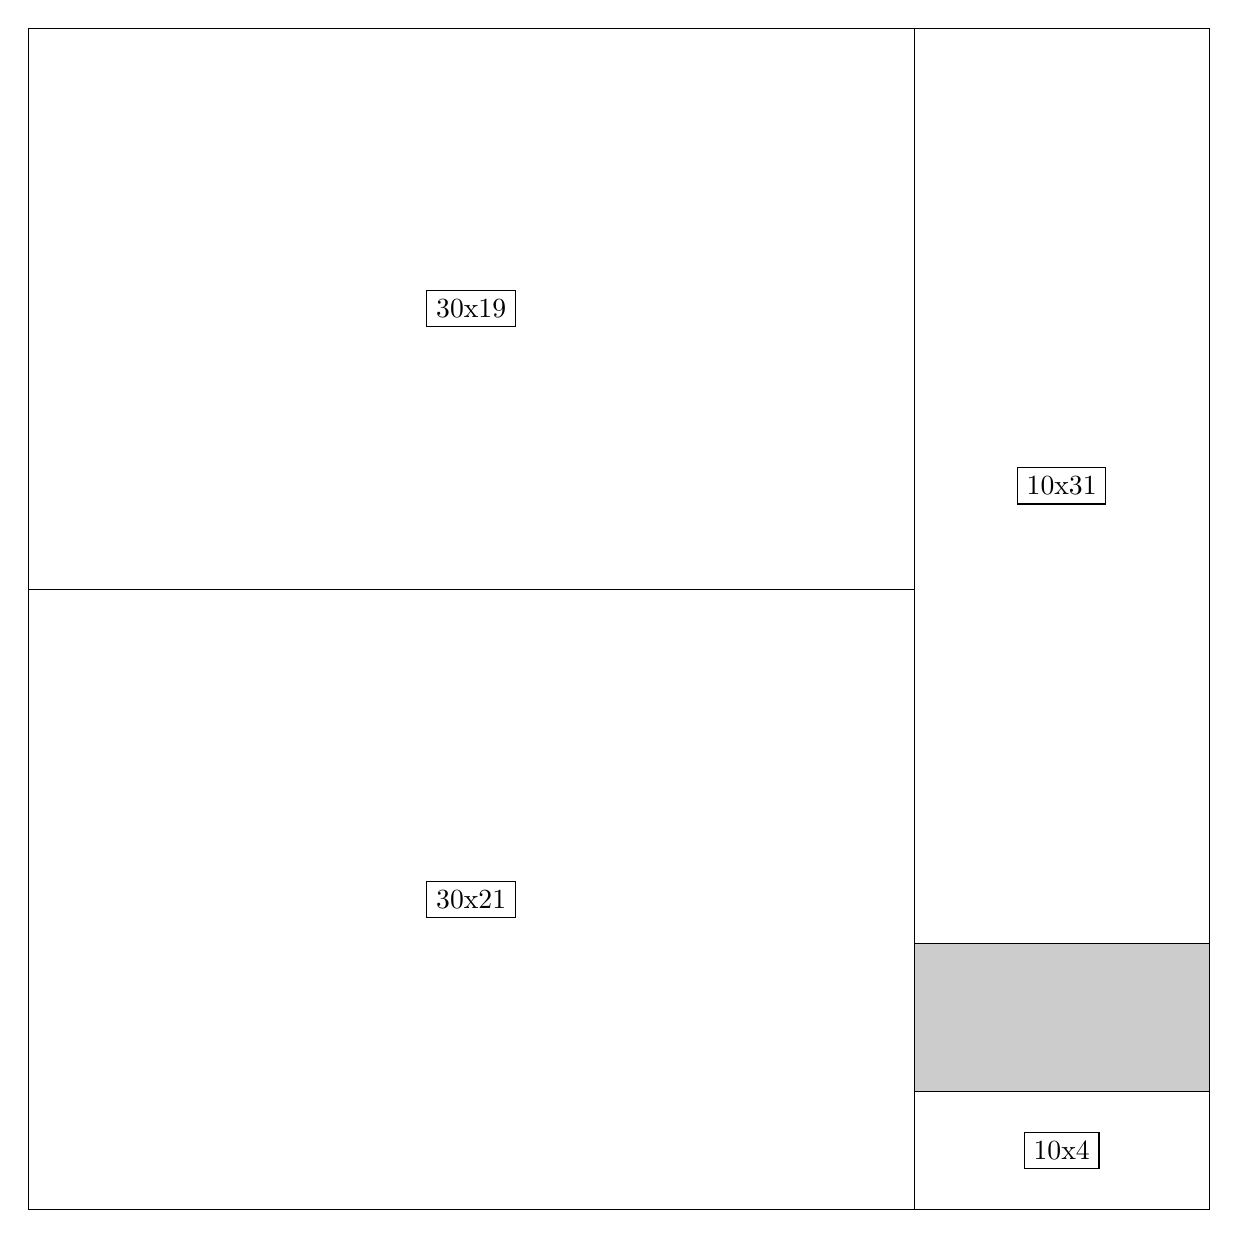
\begin{tikzpicture}[shorten >=1pt,scale=1.0,every node/.style={scale=1.0},->]
\tikzstyle{vertex}=[circle,fill=black!25,minimum size=14pt,inner sep=0pt]
\filldraw[fill=gray!40!white, draw=black] (0,0) rectangle (15.0,15.0);
\foreach \name/\x/\y/\w/\h in {30x21/0.0/0.0/11.25/7.875,30x19/0.0/7.875/11.25/7.125,10x31/11.25/3.375/3.75/11.625,10x4/11.25/0.0/3.75/1.5}
\filldraw[fill=white!40!white, draw=black] (\x,\y) rectangle node[draw] (\name) {\name} ++(\w,\h);
\end{tikzpicture}


w =30 , h =21 , x =0 , y =0 , v =630
\par
w =30 , h =19 , x =0 , y =21 , v =570
\par
w =10 , h =31 , x =30 , y =9 , v =310
\par
w =10 , h =4 , x =30 , y =0 , v =40
\par
\newpage


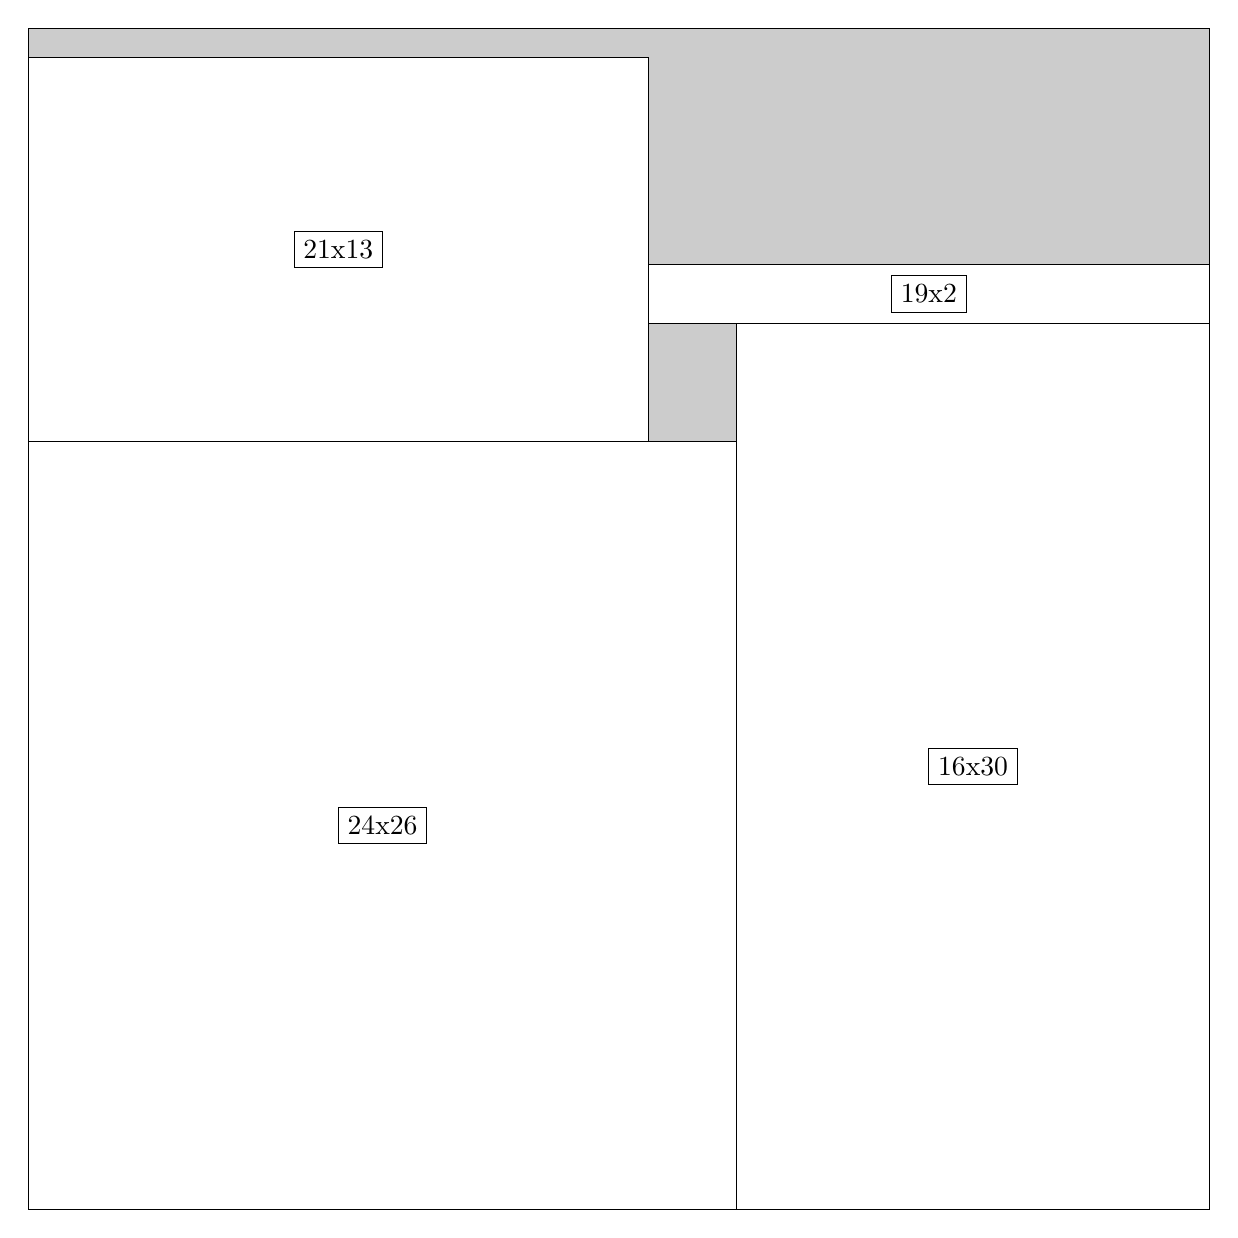
\begin{tikzpicture}[shorten >=1pt,scale=1.0,every node/.style={scale=1.0},->]
\tikzstyle{vertex}=[circle,fill=black!25,minimum size=14pt,inner sep=0pt]
\filldraw[fill=gray!40!white, draw=black] (0,0) rectangle (15.0,15.0);
\foreach \name/\x/\y/\w/\h in {24x26/0.0/0.0/9.0/9.75,16x30/9.0/0.0/6.0/11.25,21x13/0.0/9.75/7.875/4.875,19x2/7.875/11.25/7.125/0.75}
\filldraw[fill=white!40!white, draw=black] (\x,\y) rectangle node[draw] (\name) {\name} ++(\w,\h);
\end{tikzpicture}


w =24 , h =26 , x =0 , y =0 , v =624
\par
w =16 , h =30 , x =24 , y =0 , v =480
\par
w =21 , h =13 , x =0 , y =26 , v =273
\par
w =19 , h =2 , x =21 , y =30 , v =38
\par
\newpage


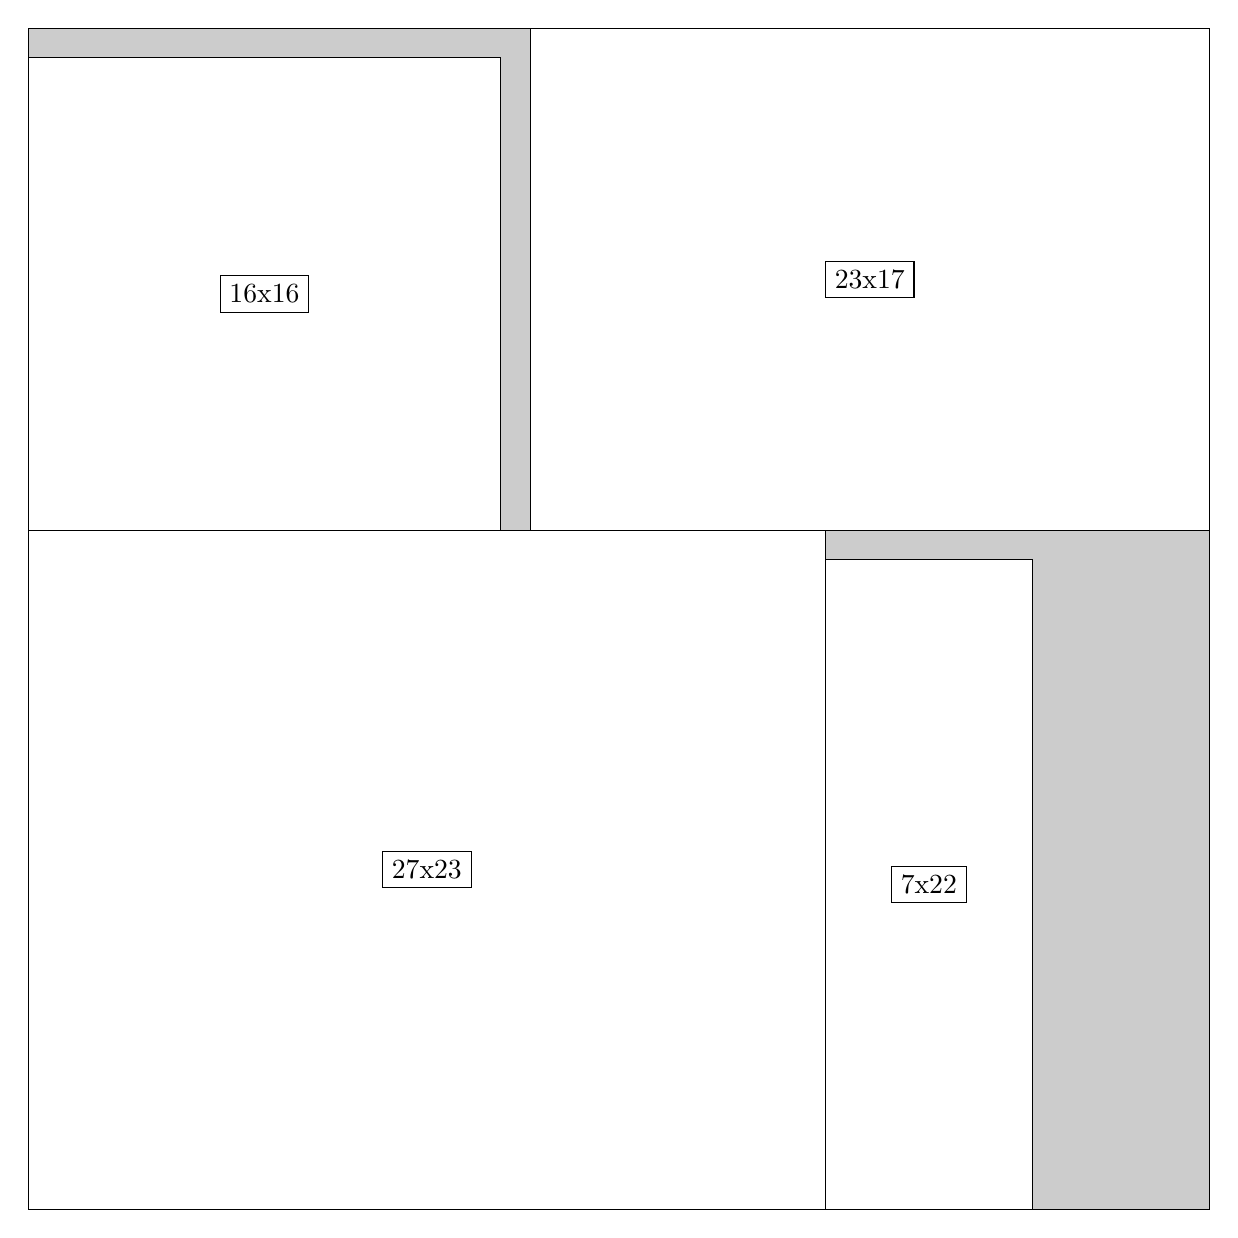
\begin{tikzpicture}[shorten >=1pt,scale=1.0,every node/.style={scale=1.0},->]
\tikzstyle{vertex}=[circle,fill=black!25,minimum size=14pt,inner sep=0pt]
\filldraw[fill=gray!40!white, draw=black] (0,0) rectangle (15.0,15.0);
\foreach \name/\x/\y/\w/\h in {27x23/0.0/0.0/10.125/8.625,23x17/6.375/8.625/8.625/6.375,16x16/0.0/8.625/6.0/6.0,7x22/10.125/0.0/2.625/8.25}
\filldraw[fill=white!40!white, draw=black] (\x,\y) rectangle node[draw] (\name) {\name} ++(\w,\h);
\end{tikzpicture}


w =27 , h =23 , x =0 , y =0 , v =621
\par
w =23 , h =17 , x =17 , y =23 , v =391
\par
w =16 , h =16 , x =0 , y =23 , v =256
\par
w =7 , h =22 , x =27 , y =0 , v =154
\par
\newpage


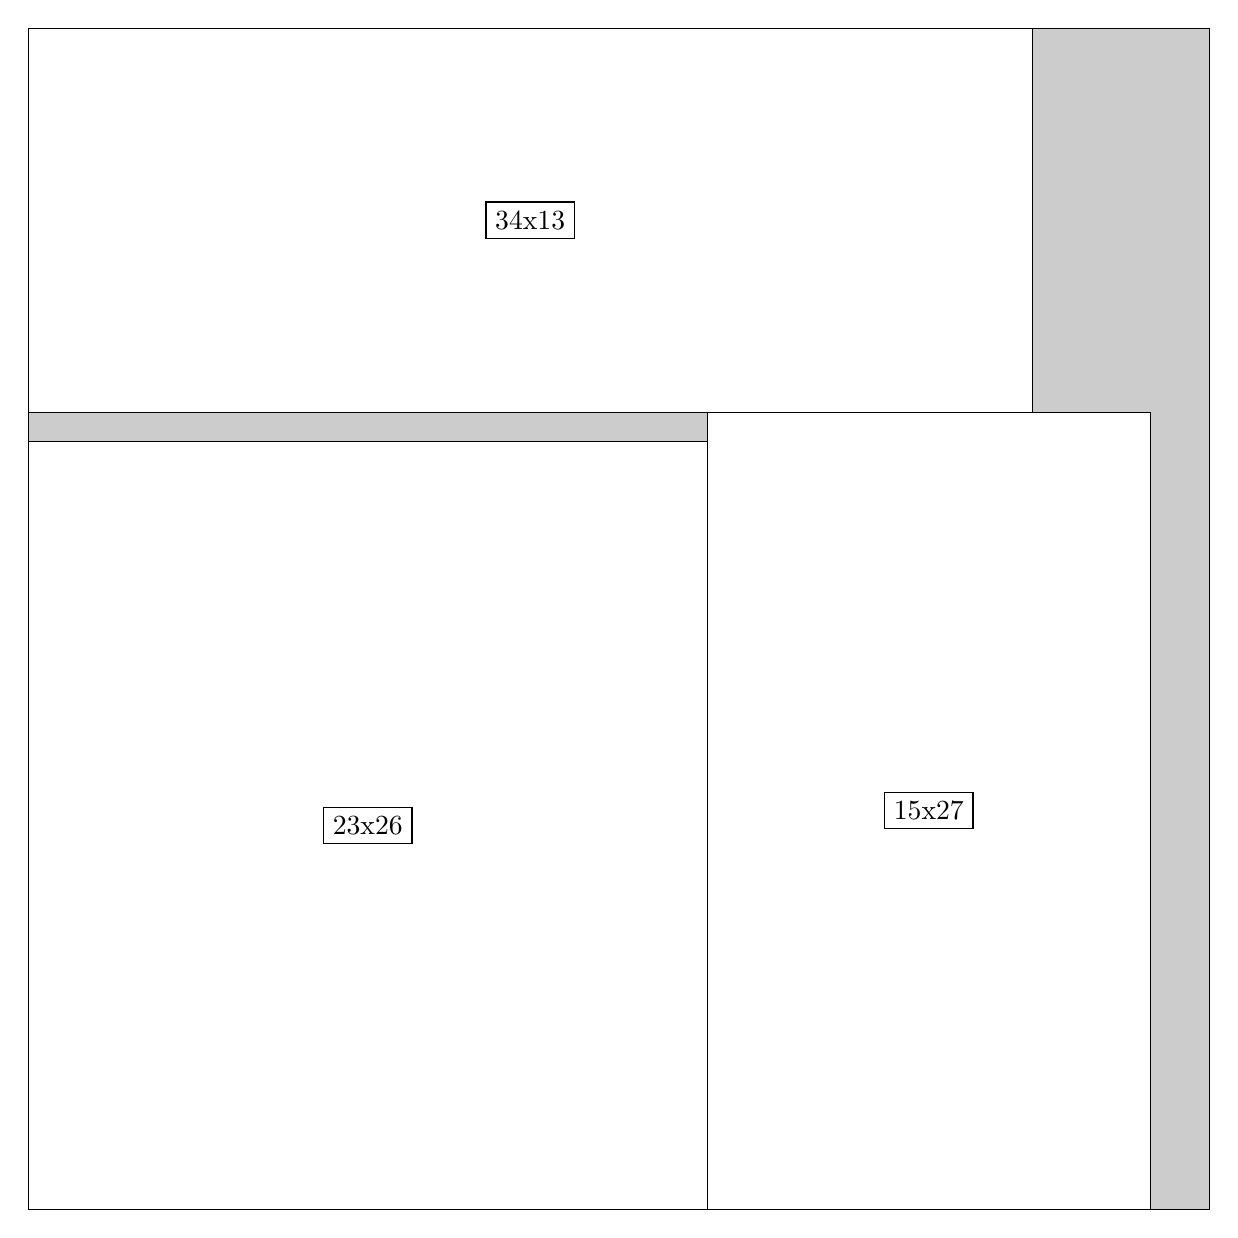
\begin{tikzpicture}[shorten >=1pt,scale=1.0,every node/.style={scale=1.0},->]
\tikzstyle{vertex}=[circle,fill=black!25,minimum size=14pt,inner sep=0pt]
\filldraw[fill=gray!40!white, draw=black] (0,0) rectangle (15.0,15.0);
\foreach \name/\x/\y/\w/\h in {23x26/0.0/0.0/8.625/9.75,34x13/0.0/10.125/12.75/4.875,15x27/8.625/0.0/5.625/10.125}
\filldraw[fill=white!40!white, draw=black] (\x,\y) rectangle node[draw] (\name) {\name} ++(\w,\h);
\end{tikzpicture}


w =23 , h =26 , x =0 , y =0 , v =598
\par
w =34 , h =13 , x =0 , y =27 , v =442
\par
w =15 , h =27 , x =23 , y =0 , v =405
\par
\newpage


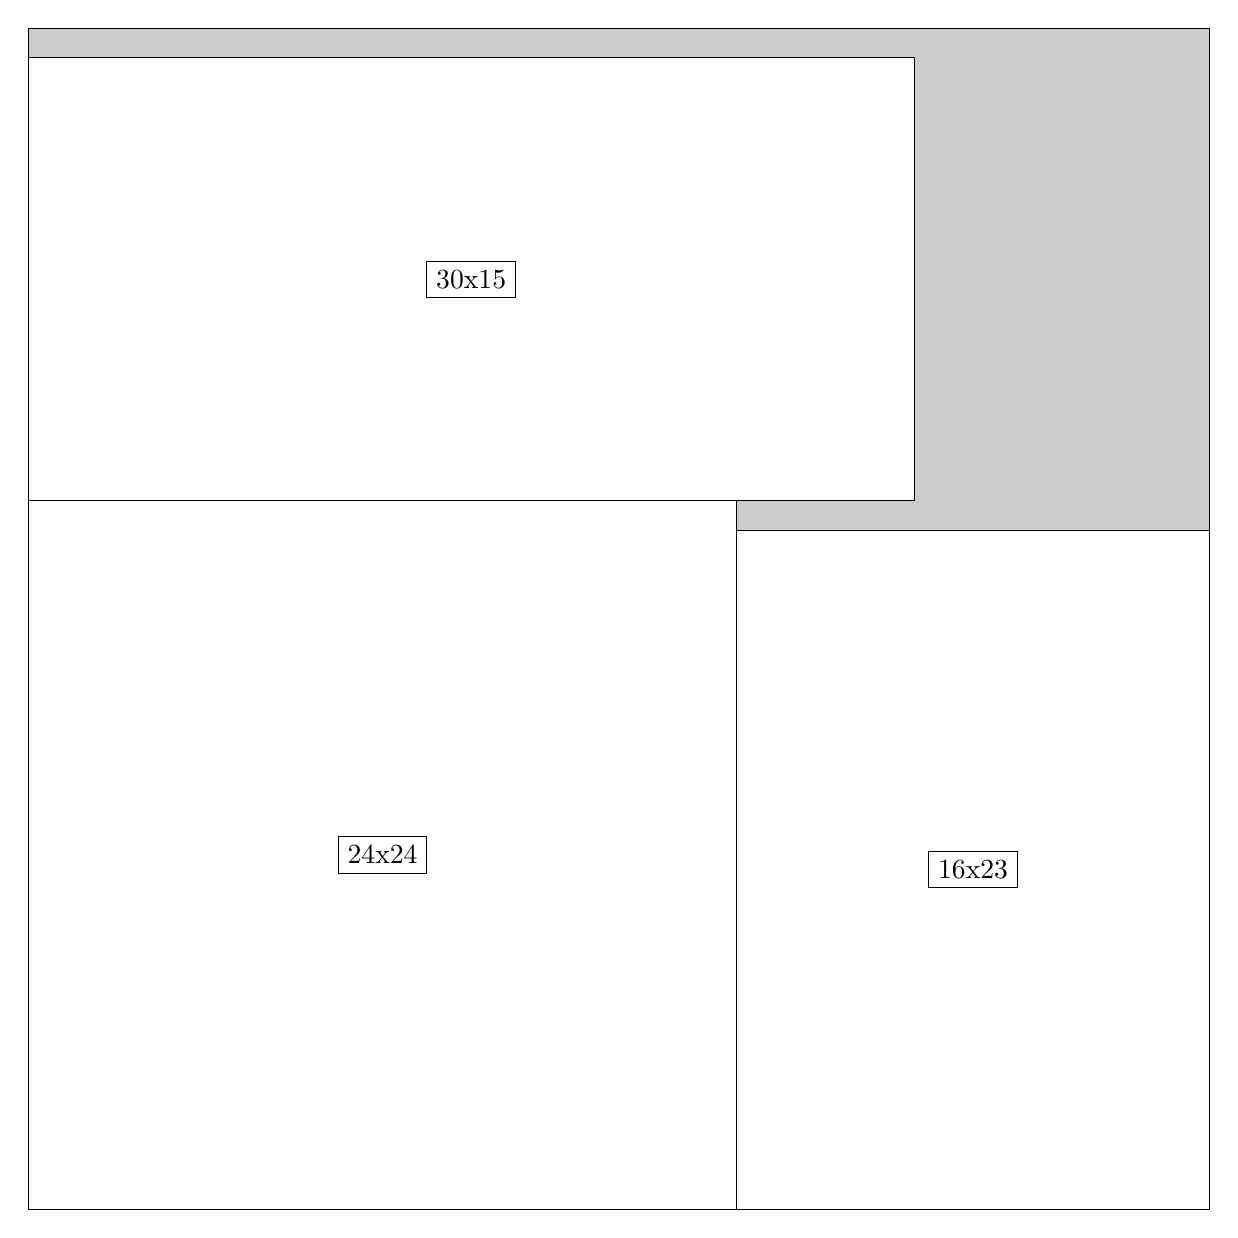
\begin{tikzpicture}[shorten >=1pt,scale=1.0,every node/.style={scale=1.0},->]
\tikzstyle{vertex}=[circle,fill=black!25,minimum size=14pt,inner sep=0pt]
\filldraw[fill=gray!40!white, draw=black] (0,0) rectangle (15.0,15.0);
\foreach \name/\x/\y/\w/\h in {16x23/9.0/0.0/6.0/8.625,30x15/0.0/9.0/11.25/5.625,24x24/0.0/0.0/9.0/9.0}
\filldraw[fill=white!40!white, draw=black] (\x,\y) rectangle node[draw] (\name) {\name} ++(\w,\h);
\end{tikzpicture}


w =16 , h =23 , x =24 , y =0 , v =368
\par
w =30 , h =15 , x =0 , y =24 , v =450
\par
w =24 , h =24 , x =0 , y =0 , v =576
\par
\newpage


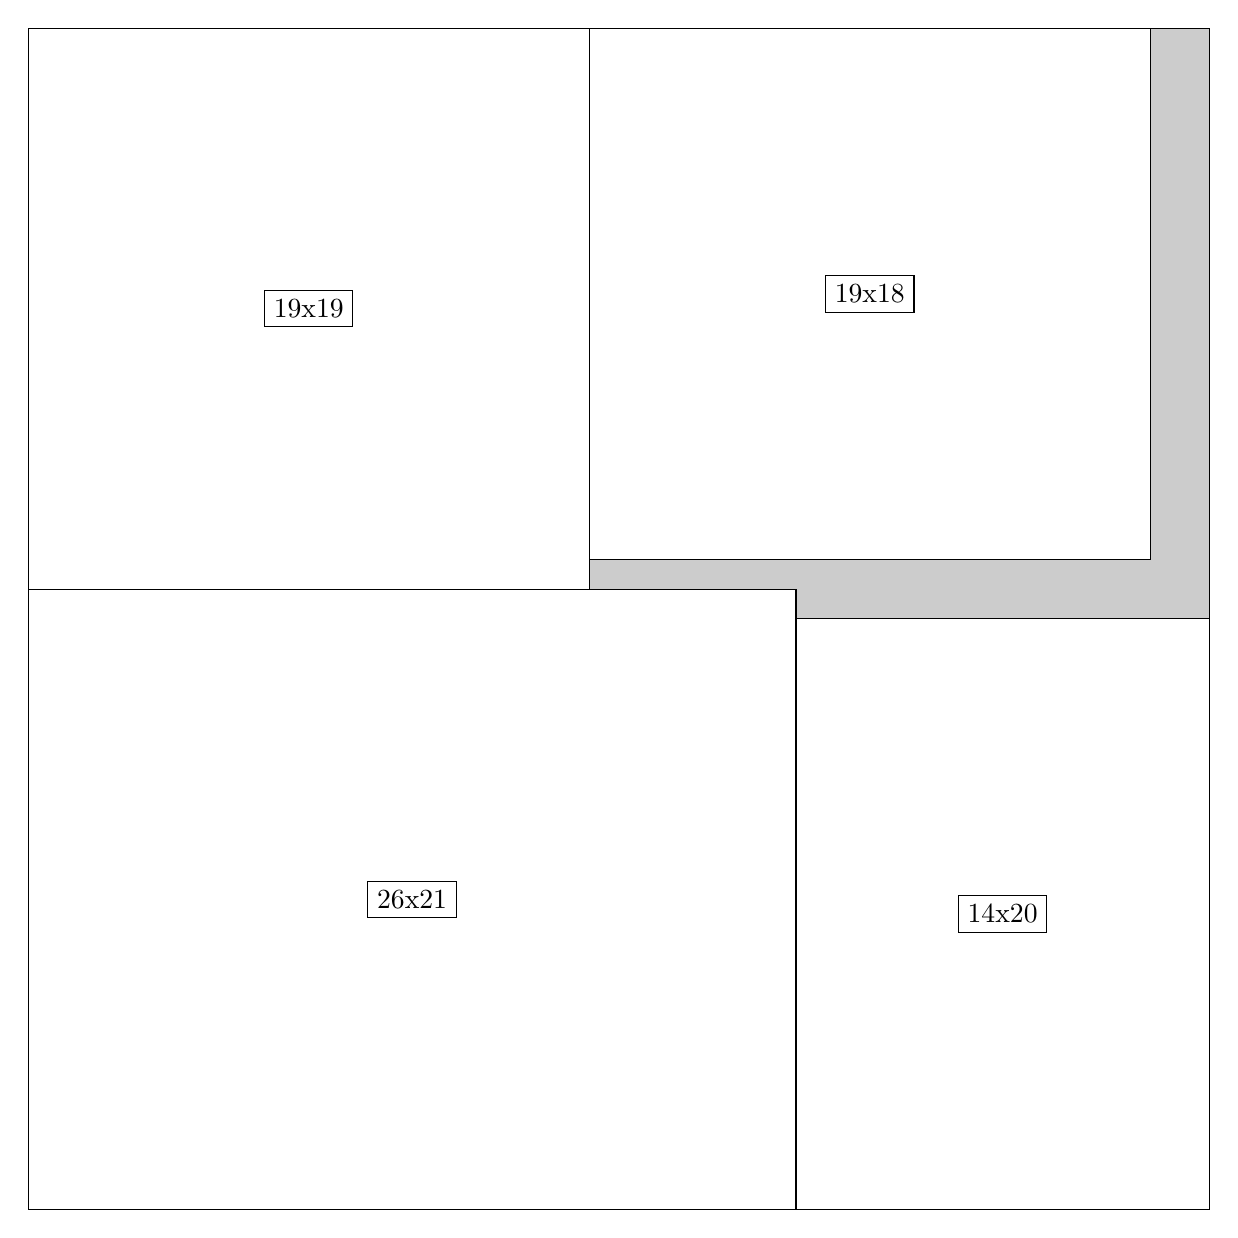
\begin{tikzpicture}[shorten >=1pt,scale=1.0,every node/.style={scale=1.0},->]
\tikzstyle{vertex}=[circle,fill=black!25,minimum size=14pt,inner sep=0pt]
\filldraw[fill=gray!40!white, draw=black] (0,0) rectangle (15.0,15.0);
\foreach \name/\x/\y/\w/\h in {26x21/0.0/0.0/9.75/7.875,19x19/0.0/7.875/7.125/7.125,19x18/7.125/8.25/7.125/6.75,14x20/9.75/0.0/5.25/7.5}
\filldraw[fill=white!40!white, draw=black] (\x,\y) rectangle node[draw] (\name) {\name} ++(\w,\h);
\end{tikzpicture}


w =26 , h =21 , x =0 , y =0 , v =546
\par
w =19 , h =19 , x =0 , y =21 , v =361
\par
w =19 , h =18 , x =19 , y =22 , v =342
\par
w =14 , h =20 , x =26 , y =0 , v =280
\par
\newpage


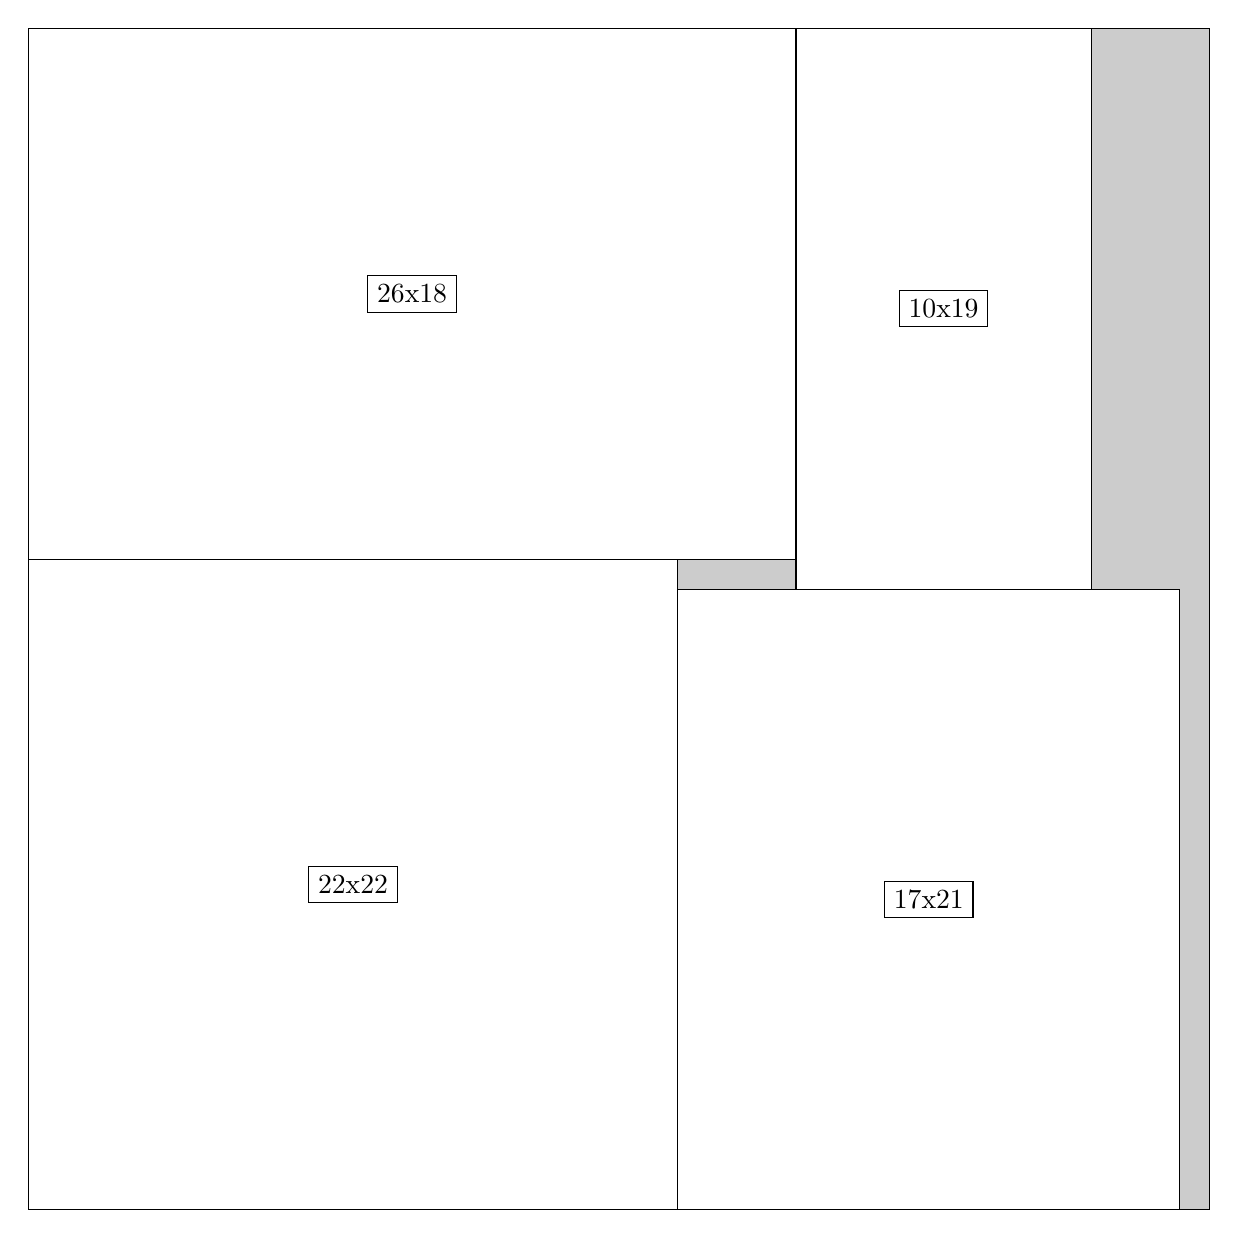
\begin{tikzpicture}[shorten >=1pt,scale=1.0,every node/.style={scale=1.0},->]
\tikzstyle{vertex}=[circle,fill=black!25,minimum size=14pt,inner sep=0pt]
\filldraw[fill=gray!40!white, draw=black] (0,0) rectangle (15.0,15.0);
\foreach \name/\x/\y/\w/\h in {22x22/0.0/0.0/8.25/8.25,26x18/0.0/8.25/9.75/6.75,17x21/8.25/0.0/6.375/7.875,10x19/9.75/7.875/3.75/7.125}
\filldraw[fill=white!40!white, draw=black] (\x,\y) rectangle node[draw] (\name) {\name} ++(\w,\h);
\end{tikzpicture}


w =22 , h =22 , x =0 , y =0 , v =484
\par
w =26 , h =18 , x =0 , y =22 , v =468
\par
w =17 , h =21 , x =22 , y =0 , v =357
\par
w =10 , h =19 , x =26 , y =21 , v =190
\par
\newpage


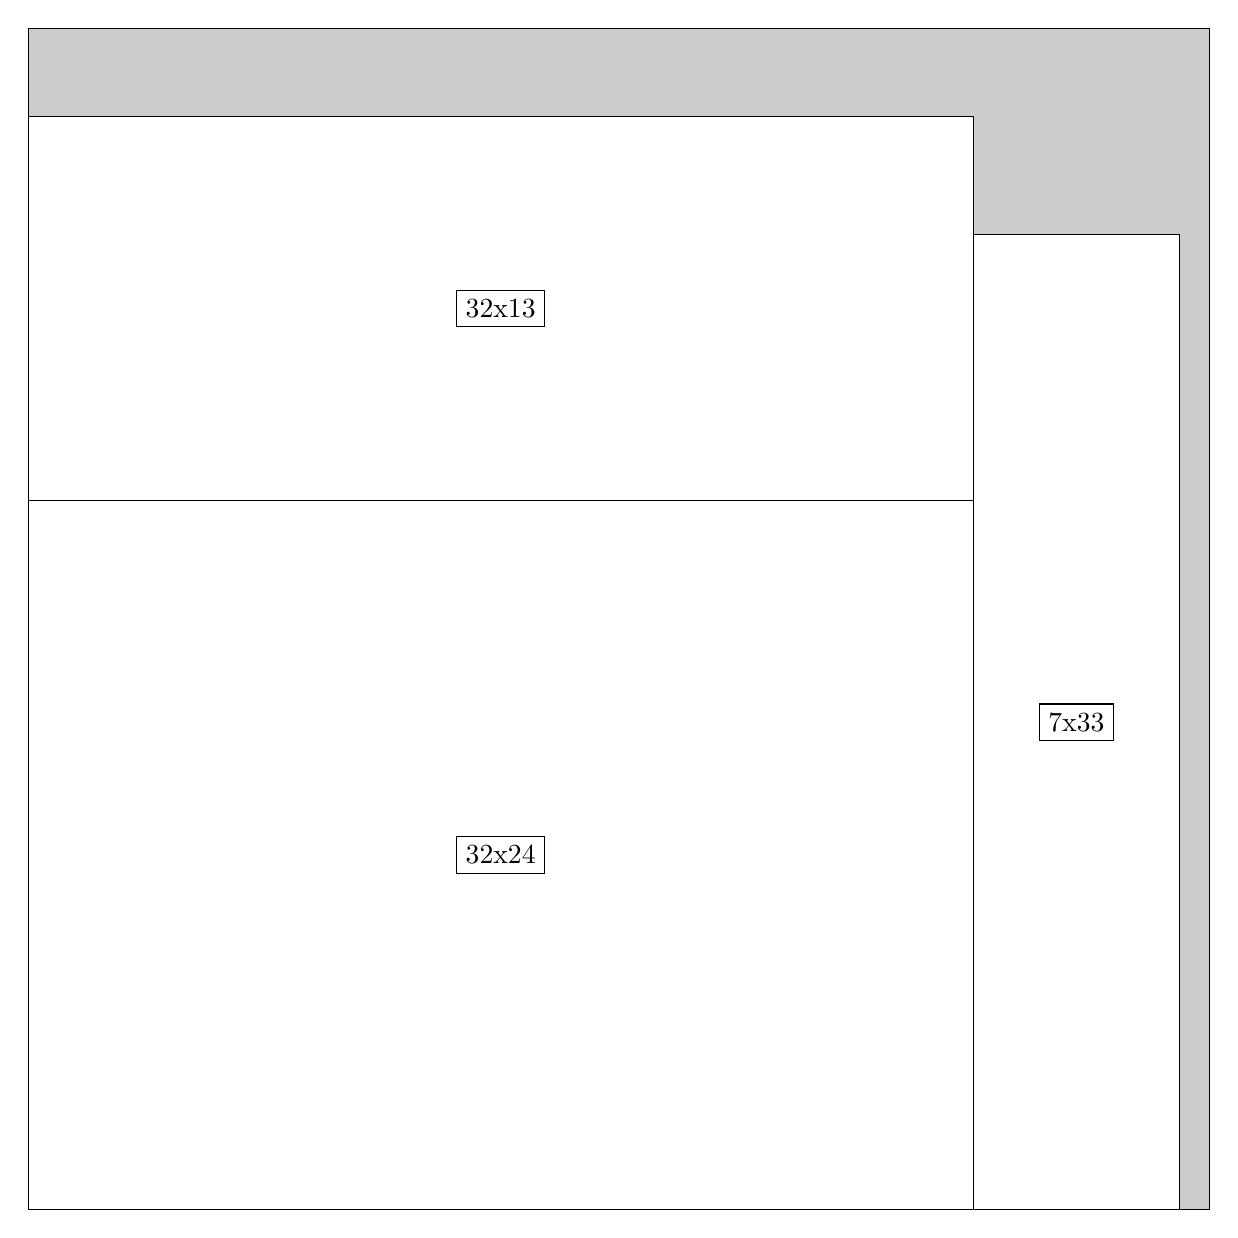
\begin{tikzpicture}[shorten >=1pt,scale=1.0,every node/.style={scale=1.0},->]
\tikzstyle{vertex}=[circle,fill=black!25,minimum size=14pt,inner sep=0pt]
\filldraw[fill=gray!40!white, draw=black] (0,0) rectangle (15.0,15.0);
\foreach \name/\x/\y/\w/\h in {32x13/0.0/9.0/12.0/4.875,7x33/12.0/0.0/2.625/12.375,32x24/0.0/0.0/12.0/9.0}
\filldraw[fill=white!40!white, draw=black] (\x,\y) rectangle node[draw] (\name) {\name} ++(\w,\h);
\end{tikzpicture}


w =32 , h =13 , x =0 , y =24 , v =416
\par
w =7 , h =33 , x =32 , y =0 , v =231
\par
w =32 , h =24 , x =0 , y =0 , v =768
\par
\newpage


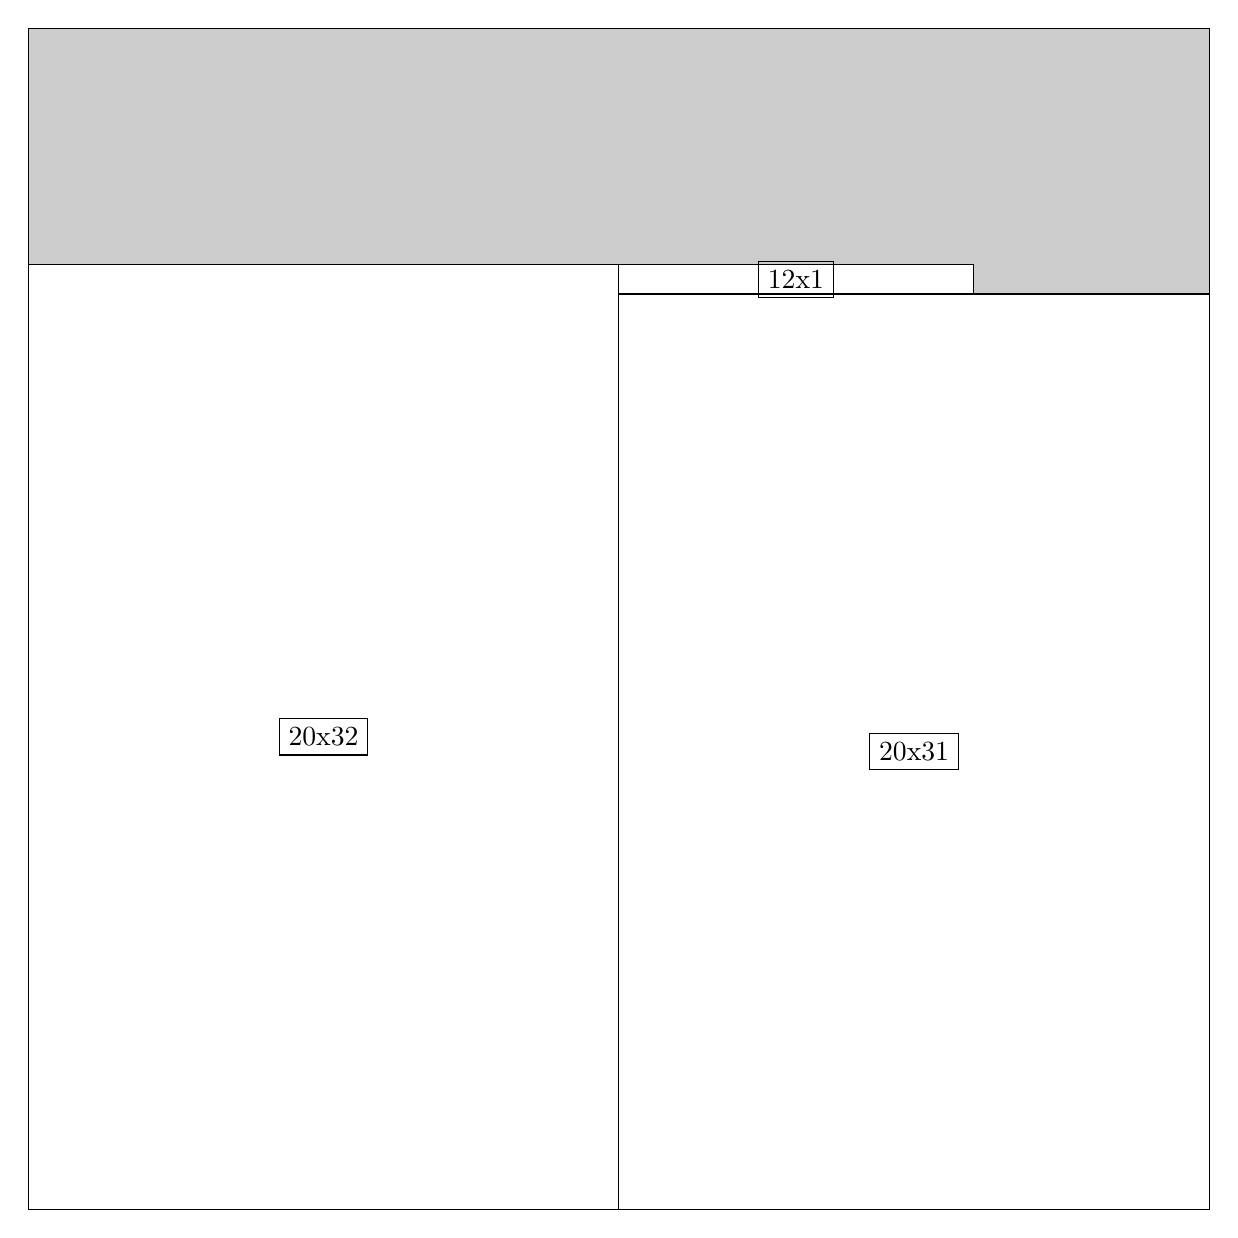
\begin{tikzpicture}[shorten >=1pt,scale=1.0,every node/.style={scale=1.0},->]
\tikzstyle{vertex}=[circle,fill=black!25,minimum size=14pt,inner sep=0pt]
\filldraw[fill=gray!40!white, draw=black] (0,0) rectangle (15.0,15.0);
\foreach \name/\x/\y/\w/\h in {20x32/0.0/0.0/7.5/12.0,20x31/7.5/0.0/7.5/11.625,12x1/7.5/11.625/4.5/0.375}
\filldraw[fill=white!40!white, draw=black] (\x,\y) rectangle node[draw] (\name) {\name} ++(\w,\h);
\end{tikzpicture}


w =20 , h =32 , x =0 , y =0 , v =640
\par
w =20 , h =31 , x =20 , y =0 , v =620
\par
w =12 , h =1 , x =20 , y =31 , v =12
\par
\newpage


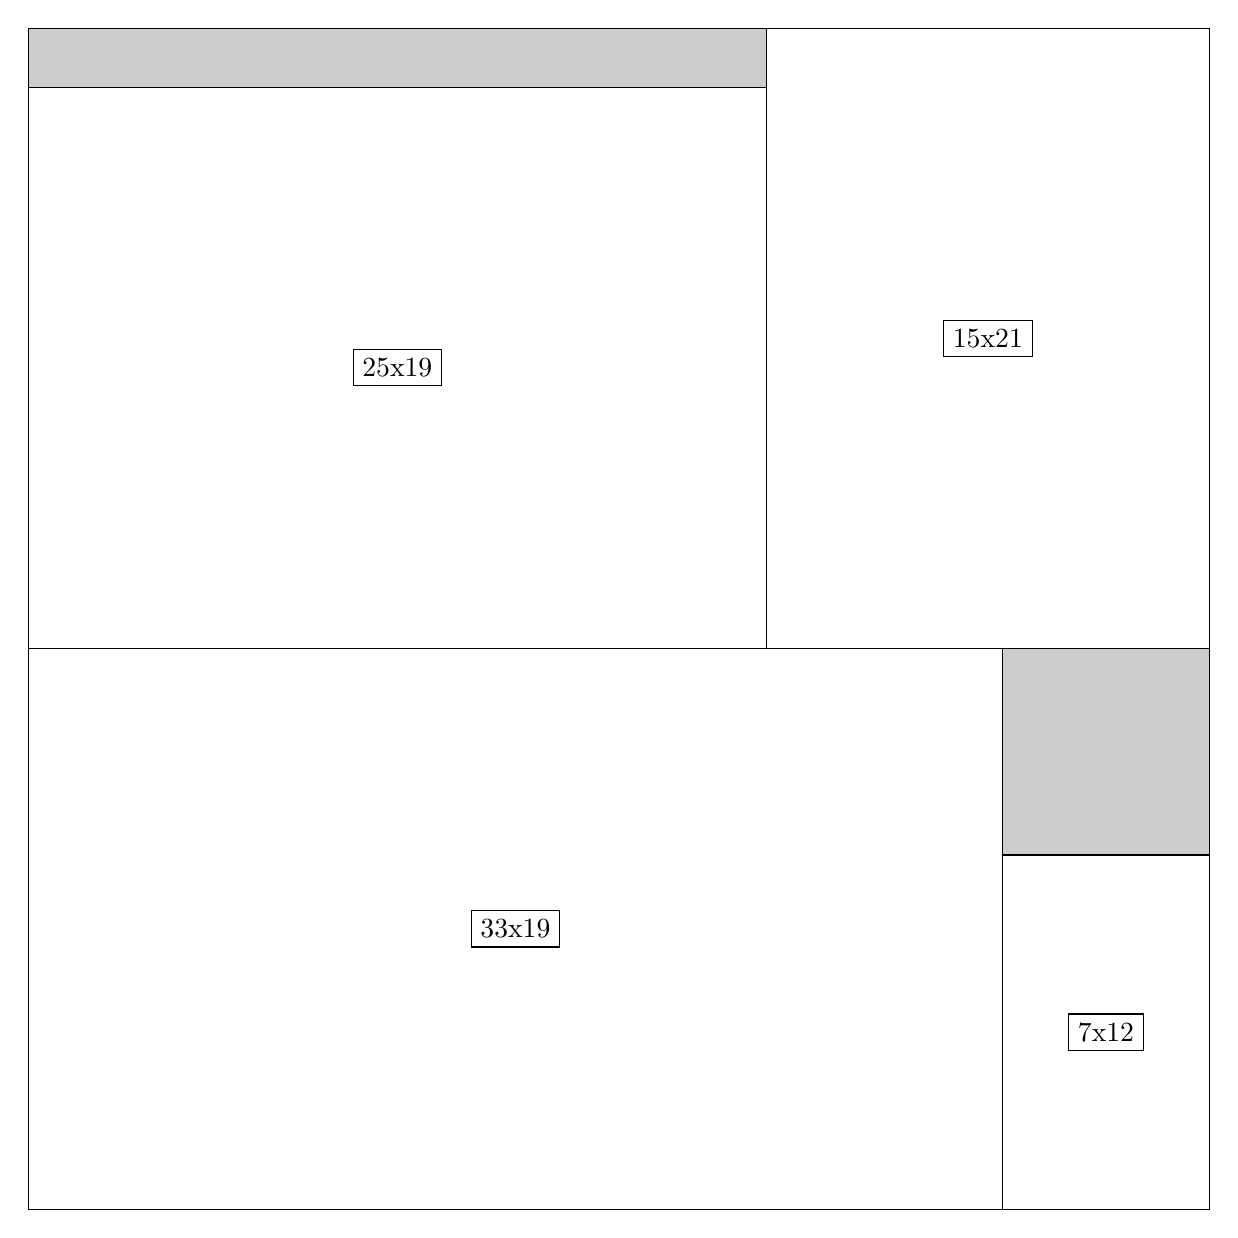
\begin{tikzpicture}[shorten >=1pt,scale=1.0,every node/.style={scale=1.0},->]
\tikzstyle{vertex}=[circle,fill=black!25,minimum size=14pt,inner sep=0pt]
\filldraw[fill=gray!40!white, draw=black] (0,0) rectangle (15.0,15.0);
\foreach \name/\x/\y/\w/\h in {33x19/0.0/0.0/12.375/7.125,25x19/0.0/7.125/9.375/7.125,15x21/9.375/7.125/5.625/7.875,7x12/12.375/0.0/2.625/4.5}
\filldraw[fill=white!40!white, draw=black] (\x,\y) rectangle node[draw] (\name) {\name} ++(\w,\h);
\end{tikzpicture}


w =33 , h =19 , x =0 , y =0 , v =627
\par
w =25 , h =19 , x =0 , y =19 , v =475
\par
w =15 , h =21 , x =25 , y =19 , v =315
\par
w =7 , h =12 , x =33 , y =0 , v =84
\par
\newpage


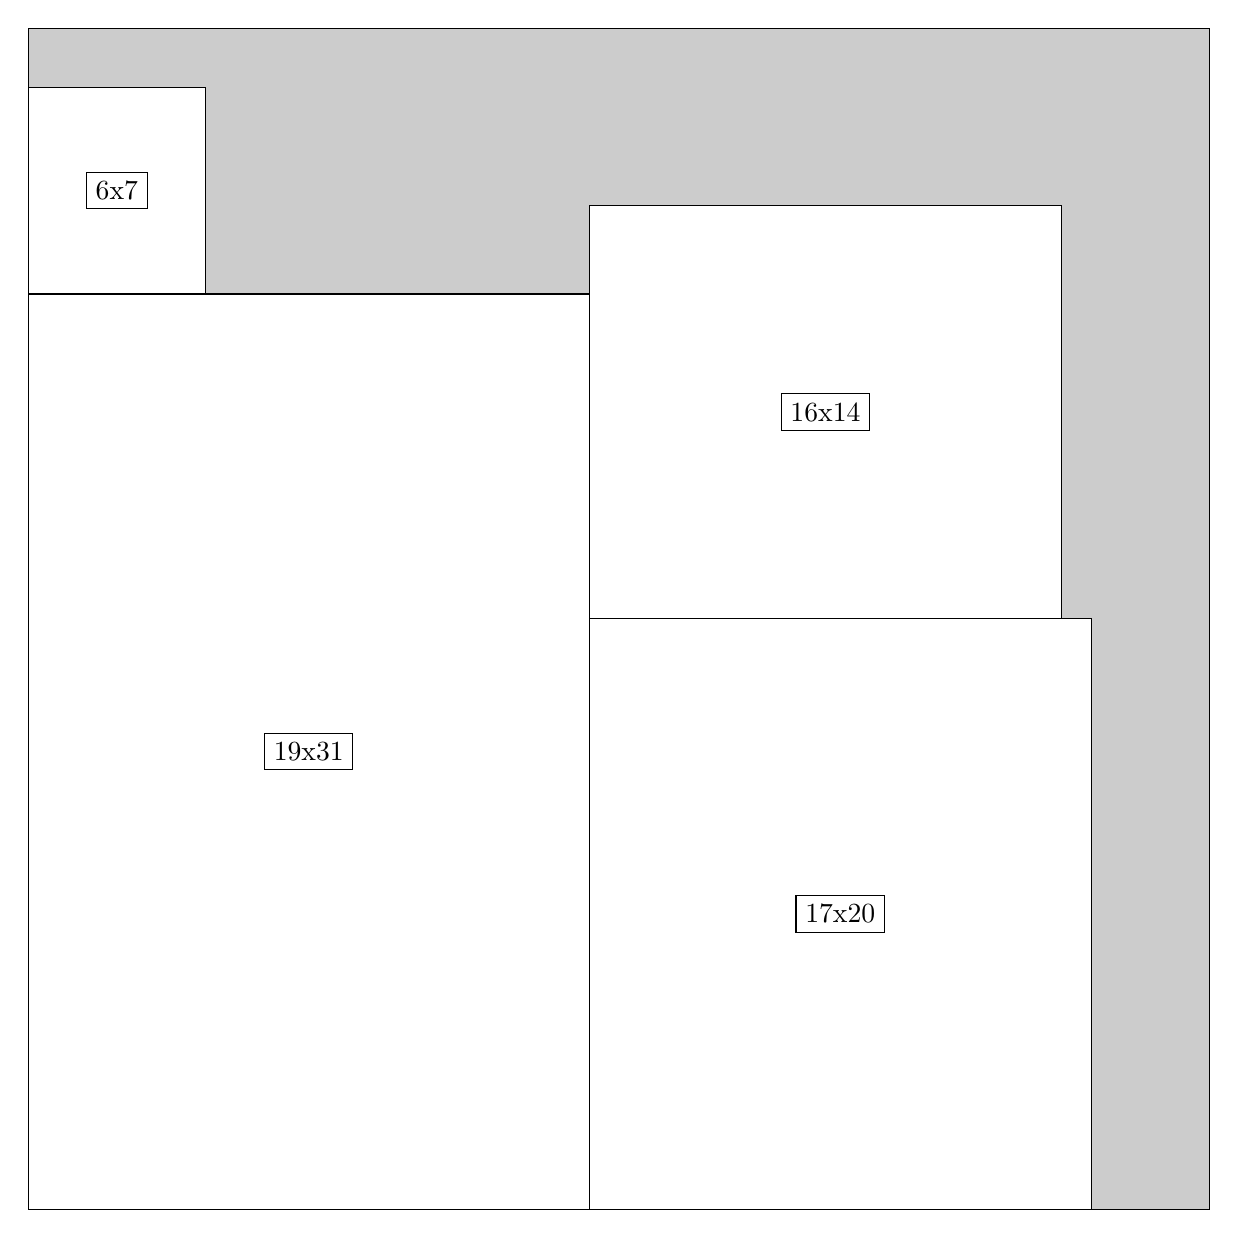
\begin{tikzpicture}[shorten >=1pt,scale=1.0,every node/.style={scale=1.0},->]
\tikzstyle{vertex}=[circle,fill=black!25,minimum size=14pt,inner sep=0pt]
\filldraw[fill=gray!40!white, draw=black] (0,0) rectangle (15.0,15.0);
\foreach \name/\x/\y/\w/\h in {19x31/0.0/0.0/7.125/11.625,17x20/7.125/0.0/6.375/7.5,16x14/7.125/7.5/6.0/5.25,6x7/0.0/11.625/2.25/2.625}
\filldraw[fill=white!40!white, draw=black] (\x,\y) rectangle node[draw] (\name) {\name} ++(\w,\h);
\end{tikzpicture}


w =19 , h =31 , x =0 , y =0 , v =589
\par
w =17 , h =20 , x =19 , y =0 , v =340
\par
w =16 , h =14 , x =19 , y =20 , v =224
\par
w =6 , h =7 , x =0 , y =31 , v =42
\par
\newpage


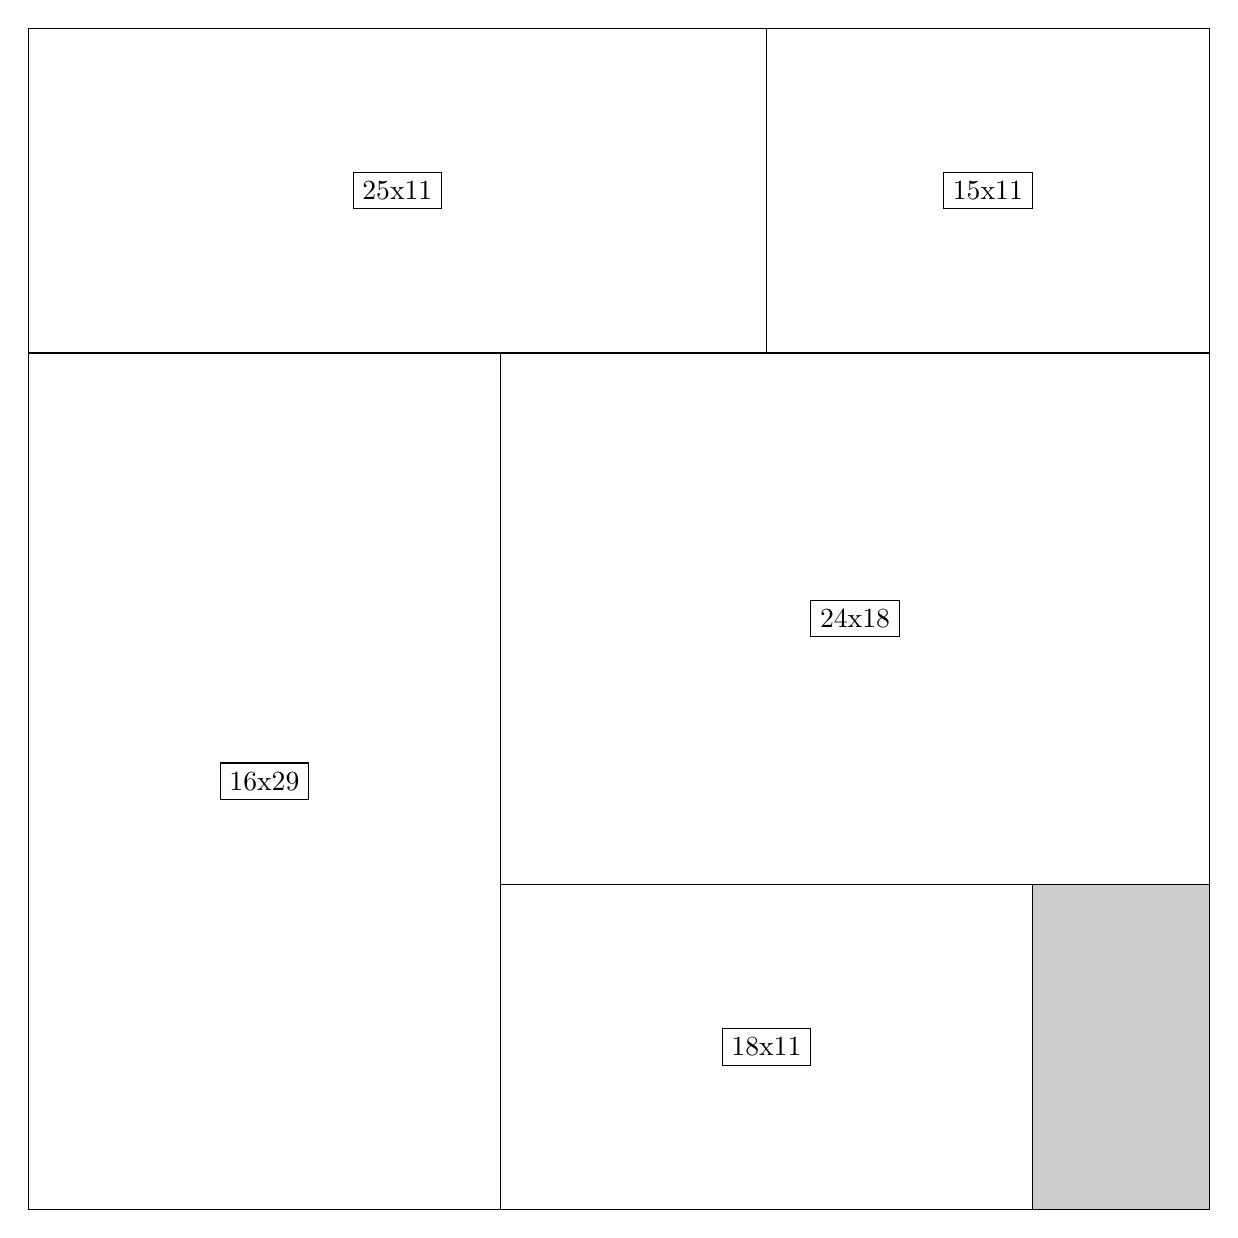
\begin{tikzpicture}[shorten >=1pt,scale=1.0,every node/.style={scale=1.0},->]
\tikzstyle{vertex}=[circle,fill=black!25,minimum size=14pt,inner sep=0pt]
\filldraw[fill=gray!40!white, draw=black] (0,0) rectangle (15.0,15.0);
\foreach \name/\x/\y/\w/\h in {16x29/0.0/0.0/6.0/10.875,24x18/6.0/4.125/9.0/6.75,25x11/0.0/10.875/9.375/4.125,18x11/6.0/0.0/6.75/4.125,15x11/9.375/10.875/5.625/4.125}
\filldraw[fill=white!40!white, draw=black] (\x,\y) rectangle node[draw] (\name) {\name} ++(\w,\h);
\end{tikzpicture}


w =16 , h =29 , x =0 , y =0 , v =464
\par
w =24 , h =18 , x =16 , y =11 , v =432
\par
w =25 , h =11 , x =0 , y =29 , v =275
\par
w =18 , h =11 , x =16 , y =0 , v =198
\par
w =15 , h =11 , x =25 , y =29 , v =165
\par
\newpage


\end{document}